\documentclass[Portugues]{ic-tese-v3}
\usepackage[utf8]{inputenc}
\usepackage{epstopdf}
\usepackage{graphicx}
\usepackage{caption}
\captionsetup{font=small,skip=3pt}
\usepackage{booktabs}
\usepackage[T1]{fontenc}
\usepackage[brazil]{babel}
\usepackage{xcolor}
\renewcommand{\topfraction}{0.9}\renewcommand{\bottomfraction}{0.8}\renewcommand{\textfraction}{0.07}\renewcommand{\floatpagefraction}{0.85}
\setlength{\textfloatsep}{8pt plus 2pt minus 2pt}\setlength{\floatsep}{6pt plus 2pt minus 2pt}\setlength{\abovecaptionskip}{3pt}
\usepackage{fancyhdr}
\usepackage{amsmath}
\usepackage[ttscale=.875]{libertine}
\usepackage{libertinust1math}
\usepackage{tabularx}
\usepackage{titlesec}
\usepackage{alltt}
\titlespacing*{\section}{0pt}{1.6ex}{0.8ex}
\definecolor{chgbluetext}{HTML}{1565C0}
\graphicspath{{figures/}}

% same margins as the computer vision report template
\geometry{reset,a4paper,left=0.75in,top=0.9in,textwidth=40pc,textheight=58.5pc,headheight=0pt,headsep=0pt}
\parindent 0.2in

\usepackage[colorlinks,linkcolor=chgbluetext,citecolor=black,urlcolor=chgbluetext]{hyperref}

\providecommand{\resetlang}{} % ponytail: used by ic-tese-v3.cls but never defined there
\newcommand{\dd}{-{}-} % ponytail: double hyphen of command-line options without a TeX ligature
\DeclareRobustCommand{\_}{\textunderscore\allowbreak} % ponytail: let long identifiers break after _
\sloppy

\begin{document}

\paginasiniciais
% ponytail: ic-tese-v3 maps plain to empty, so number pages with fancyhdr (centered footer)
\pagestyle{fancy}\fancyhf{}\fancyfoot[C]{\thepage}\renewcommand{\headrulewidth}{0pt}\thispagestyle{fancy}
\vspace{-16mm}
\begin{center}
{\large\textbf{Multiplicação de Matrizes em Blocos: Serial, MPI e MPI com OpenBLAS | MO652}}\\[2mm]
\small
\begin{tabular}{|l||c||l|}
 \hline
 Nome & RA & Email \\
 \hline\hline
 Mateus Oliveira da Silva & 203656 & m203656@dac.unicamp.br \\
 \hline
\end{tabular}
\end{center}

% Fontes de todos os números: repositório HPC_Matrix_Multiplication, pasta results/
% (benchmark.csv, metrics.csv, node_sweep.csv, saturation.csv, validation_summary.csv, logs/).

\section{Introdução e objetivo}
Este trabalho multiplica duas matrizes quadradas $N\times N$ em ponto flutuante de precisão simples, isto é, \texttt{float} de 32 bits, e calcula $C = A\cdot B$ em três versões: Serial, MPI e MPI + OpenBLAS. O objetivo é comparar as três versões no cluster Lovelace do CENAPAD/UNICAMP para $N = 2000$, 4000 e 6000, variando o tamanho do bloco, o número de processos MPI e o número de nós, e analisar a escalabilidade forte e a fraca. Todas as medições foram feitas no Lovelace. O código, os scripts PBS, os CSV e os logs estão no repositório \href{https://github.com/oliveiraMats2/HPC_Matrix_Multiplication}{github.com/\allowbreak oliveiraMats2/\allowbreak HPC\_Matrix\_\allowbreak Multiplication}.

\section{Implementação}
O programa é escrito em C11, e cada versão é um executável próprio, compilado do mesmo código, como resume a Tabela~\ref{tab:versoes}. As três versões recebem exatamente as mesmas $A$ e $B$, geradas com semente fixa.

\begin{table}[!htb]
\centering\footnotesize
\renewcommand{\arraystretch}{1.05}
\begin{tabularx}{\textwidth}{|l|l|c|X|}
\hline
\textbf{Versão} & \textbf{Executável} & \textbf{Processos} & \textbf{Kernel local dos blocos} \\
\hline\hline
Serial & \texttt{matmul\_serial} & 1 & laço i-k-j em ladrilhos $b\times b$, em C puro, \texttt{kernel\_naive}, sem BLAS \\ \hline
MPI & \texttt{matmul\_mpi} & $p$ & o mesmo laço em ladrilhos em C puro, sem BLAS \\ \hline
MPI + OpenBLAS & \texttt{matmul\_mpi\_openblas} & $p$ & uma chamada \texttt{cblas\_sgemm} por trio de ladrilhos, \texttt{kernel\_openblas}; OpenBLAS com 1 thread \\ \hline
\end{tabularx}
\caption{As três versões. MPI e MPI + OpenBLAS usam o mesmo motor de distribuição, \texttt{mpi\_distributed\_multiply()}; só o kernel local muda.}
\label{tab:versoes}
\end{table}

\textbf{Serial.} Executa em um único processo, sem MPI e sem BLAS. O produto é calculado em ladrilhos $b\times b$ com o laço i-k-j; o laço mais interno tem passo 1 e é vetorizado pelo compilador.

\textbf{Distribuição MPI.} As duas versões MPI usam a distribuição por faixas de linhas, \texttt{row\_block}. O processo 0 tem $A$, $B$ e $C$ globais. A matriz $A$ é dividida em faixas contíguas de linhas por \texttt{MPI\_Scatterv}, e o rank $r$ recebe $m_r$ linhas, com
\begin{equation}\label{eq:linhas}
m_r \in \left\{ \left\lfloor \frac{N}{p} \right\rfloor, \left\lceil \frac{N}{p} \right\rceil \right\},
\qquad \sum_{r=0}^{p-1} m_r = N,
\end{equation}
em que $p$ é o número de processos MPI e $r = 0, \dots, p-1$ é o índice do rank. As alturas diferem, portanto, de no máximo uma linha, e $N$ não precisa ser divisível por $p$: os vetores de contagens e deslocamentos do \texttt{Scatterv} absorvem o resto, e um rank sem linhas, quando $p>N$, apenas não chama o kernel. Todo rank recebe uma cópia completa de $B$ por \texttt{MPI\_Bcast}. Cada rank calcula a sua faixa de $C$ com o kernel local, e as faixas são reunidas no rank 0 por \texttt{MPI\_Gatherv}. O rank 0 trabalha no lugar, com \texttt{MPI\_IN\_PLACE}, e os demais alocam a sua faixa de $A$, a cópia de $B$ e a faixa de $C$ antes do início do relógio.
% fonte: src/algorithms/mpi_distribution.c:82-107 (Barrier, Scatterv, Bcast, kernel, Gatherv)

\textbf{MPI + OpenBLAS.} Usa o mesmo motor de distribuição, que recebe o kernel local como parâmetro. O kernel \texttt{kernel\_openblas} faz uma chamada \texttt{cblas\_sgemm} por trio de ladrilhos, isto é, $C_{ij} \mathrel{+}= A_{ik}B_{kj}$, com $\beta=0$ no primeiro bloco de $k$. Como a comunicação é idêntica nas duas versões MPI, a diferença de tempo medida entre elas se deve só ao kernel local.

\textbf{O que é um bloco.} Há dois níveis de bloco. O primeiro, o bloco de distribuição, é a faixa de linhas de cada rank; a sua altura $m_r$, dada pela Equação~\eqref{eq:linhas}, é fixada por $N$ e $p$ e não é um parâmetro livre. O segundo, o bloco de cálculo ou tamanho de bloco $b$, é a aresta do ladrilho $b\times b$ do kernel local, configurável em \texttt{config.toml}; é este o parâmetro variado nos experimentos, com $b = 64$, 256 e 1024. Em \texttt{float}, um ladrilho de 64 ocupa 16 KiB, da ordem do L1; um de 256 ocupa 256 KiB, menos que o L2 de 512 KiB por núcleo do EPYC 7662; e um de 1024 ocupa 4 MiB, uma fração do L3. Ladrilhos de borda são menores quando $b$ não divide a dimensão. Para \texttt{kernel\_naive} o ladrilhamento não muda o resultado: para cada elemento de $C$ os produtos continuam somados em ordem crescente de $k$, por isso Serial e MPI dão resultados idênticos bit a bit para qualquer $b$ e $p$.

\section{Ambiente experimental}
A Tabela~\ref{tab:amb} resume o hardware, o software e a grade de parâmetros. Todas as medições usaram o mesmo modelo de CPU, AMD EPYC 7662, inclusive a referência serial, de modo que speedup e eficiência comparam o mesmo processador.

\begin{table}[!htb]
\centering\small
\renewcommand{\arraystretch}{1.15}
% fonte: benchmark.csv (colunas queue, hostnames, cpu_model, cpu_mismatch, modules, compiler, cflags,
% mpi_version, openblas_version, openblas_threads, omp_threads, seed), logs/1034860_single_node/environment.log,
% scripts/env_lovelace.sh, scripts/run_benchmarks.sh, scripts/*.pbs, config.toml, README.md (512 GB por nó)
% fonte (Interconexão): logs/1034858_multi_node/environment.log:90-101 (MCA btl/pml, ucx 1.21.0, /opt/pub/hpcx/hpcx-v2.50-...);
% nenhum ibstat, ibv_devinfo, lspci ou nome de HCA em results/logs
\begin{tabularx}{\textwidth}{@{}lX@{}}
\toprule
\multicolumn{2}{@{}l}{\textbf{Ambiente}} \\
\midrule
Cluster & Lovelace, CENAPAD/UNICAMP \\
Hardware por nó & 2 processadores AMD EPYC 7662, 128 núcleos e 512 GB de memória \\
Software & GCC 9.4.0, Open MPI 4.1.1 e OpenBLAS 0.3.21 \\
Alocação & Nós exclusivos; 1 processo MPI por núcleo e 1 thread por processo \\
\midrule
\multicolumn{2}{@{}l}{\textbf{Parâmetros}} \\
\midrule
Matrizes & Quadradas, de precisão simples (32 bits), com valores em $[0,1)$ \\
Dimensões e blocos & $N = 2000$, 4000 e 6000; $b = 64$, 256 e 1024 \\
Escalabilidade forte & 1 a 128 processos em potências de 2, em 1 nó; 256, 512 e 1024 processos em 2, 4 e 8 nós \\
Varredura de nós & 128 processos fixos, distribuídos em 1, 2, 4 e 8 nós \\
Escalabilidade fraca & $(N,p) = (2000,1)$, $(4000,8)$ e $(6000,27)$, em 1 nó \\
Repetições & 5 medições por configuração, cada uma precedida de 1 aquecimento descartado \\
\bottomrule
\end{tabularx}
\caption{Resumo do ambiente experimental e dos parâmetros avaliados.}
\label{tab:amb}
\end{table}

\textbf{Threads do OpenBLAS.} O número de threads do OpenBLAS foi fixado explicitamente em 1, de quatro formas redundantes: \texttt{export OPENBLAS\_NUM\_THREADS=1} e \texttt{export OMP\_NUM\_THREADS=1} em \texttt{scripts/env\_lovelace.sh}, carregado por todo job PBS; as mesmas variáveis passadas a cada rank, em cada nó, por \texttt{env} na linha do \texttt{mpirun}; \texttt{threads = 1} na seção \texttt{[openblas]} do \texttt{config.toml}, aplicado com \texttt{openblas\_set\_num\_threads()}; e o valor que o OpenBLAS informa depois disso, gravado em cada linha do CSV: \texttt{openblas\_threads = 1} nas 1350 linhas de MPI + OpenBLAS e \texttt{omp\_threads = 1} nas 2790 linhas. Com 1 processo MPI por núcleo, fixado por \texttt{\dd bind-to core}, o número de processos é igual ao número de núcleos ocupados; não houve experimento variando threads.

\textbf{Nós exclusivos e filas.} Toda medição usou nós inteiros e exclusivos, inclusive a Serial, que roda dentro do job \texttt{par128} com 1 núcleo ocupado e os outros 127 ociosos. Um nó usa a fila \texttt{par128}; 2 a 8 nós usam a fila \texttt{paralela}. Cada job registra o modelo de CPU de cada host, e as linhas de outro modelo seriam marcadas \texttt{cpu\_mismatch} e excluídas; nenhuma foi. Os três jobs de medição terminaram com 0 lançamentos com falha.

\textbf{Ordem das execuções.} Contra o ruído temporal, as execuções foram intercaladas por rodada: a rodada 1 executa todas as combinações de versão, $N$, $b$ e $p$, depois a rodada 2, e assim por diante até a rodada 5. Cada lançamento do \texttt{mpirun} faz 1 aquecimento descartado e 1 execução medida.

\section{Procedimento de medição}\label{sec:proc}
\textbf{Etapas medidas.} O relógio é \texttt{clock\_gettime(CLOCK\_MONOTONIC)}. Nas versões MPI há um \texttt{MPI\_Barrier} imediatamente antes do instante $t_0$; depois vêm o \texttt{Scatterv} de $A$ e o \texttt{Bcast} de $B$, até $t_1$, o kernel local, até $t_2$, e o \texttt{Gatherv} de $C$, até $t_3$. Os tempos das etapas são
\begin{equation}\label{eq:fases}
t_{\mathrm{dist}} = t_1 - t_0, \qquad
t_{\textrm{cálculo}} = t_2 - t_1, \qquad
t_{\mathrm{col}} = t_3 - t_2, \qquad
t_{\mathrm{total}} = t_3 - t_0,
\end{equation}
em que $t_{\mathrm{dist}}$ é a distribuição, $t_{\textrm{cálculo}}$ o cálculo local, $t_{\mathrm{col}}$ a coleta e $t_{\mathrm{total}}$ o tempo total. Na Serial só o kernel é medido, com $t_{\mathrm{dist}} = t_{\mathrm{col}} = 0$. Ficam fora da medição a inicialização do MPI, a geração das matrizes, a alocação dos buffers, cujas páginas são tocadas antes de $t_0$, a geração ou leitura da referência e a validação.

\textbf{Máximo entre ranks.} Cada um dos quatro tempos é reduzido com \texttt{MPI\_Reduce} e \texttt{MPI\_MAX} no rank 0, de forma independente:
\begin{equation}\label{eq:max}
t_x = \max_{0 \le r < p} t_x^{(r)}, \qquad x \in \{\textrm{distribuição},\ \textrm{cálculo},\ \textrm{coleta},\ \mathrm{total}\},
\end{equation}
em que $t_x^{(r)}$ é o tempo da etapa $x$ medido no rank $r$. O tempo total relatado é, portanto, o do rank mais lento, e como cada máximo é tomado separadamente, os máximos das fases não precisam somar o total.

\textbf{Validação fora do tempo.} A validação roda no rank 0 depois da redução, com cronômetro próprio, gravado em \texttt{time\_validation\_s}. Os tempos, speedups, eficiências e GFLOP/s apresentados excluem a validação.

\textbf{Repetições e estatística.} Cada configuração tem 5 execuções medidas, uma por rodada, e os aquecimentos são descartados: são 1395 execuções medidas e 1395 aquecimentos, 2790 linhas no total, em 279 configurações. A medida representativa $T$ é a mediana das 5 execuções; a variabilidade é dada pelo desvio padrão amostral $\sigma$ e pelo intervalo interquartil, IQR. Nas tabelas, o formato ``mediana (desvio)'' indica a mediana com o desvio padrão entre parênteses. Como medida de dispersão relativa usa-se o coeficiente de variação,
\begin{equation}\label{eq:cv}
\mathrm{CV} = \frac{\sigma}{\bar{t}},
\end{equation}
em que $\sigma$ é o desvio padrão amostral e $\bar{t}$ a média das 5 execuções de uma configuração. Sobre as 279 configurações, o CV mediano do tempo total é 0,94\,\% e o IQR/mediana mediano é 0,84\,\%; 28 configurações têm CV acima de 5\,\% e 11 acima de 10\,\%. O maior caso é MPI + OpenBLAS com $N=2000$, $b=64$ e $p=512$, com desvio/mediana de até 566\,\% e CV de até 161\,\%: uma das 5 execuções levou 0,9037 s contra cerca de 0,065 s das outras, e o excesso está todo na distribuição. Outros casos isolados do mesmo tipo ocorreram no job multinó 1034858. A mediana e o IQR são robustos a esses valores isolados; o desvio padrão não.
% fonte: results/benchmark.csv, warmup=false, time_total_s agrupado por (algorithm, matrix_size, block_size, processes, nodes, scaling):
% 279 grupos; std/mediana e std/média têm a mesma mediana (0,94 %) e as mesmas contagens (28 > 5 %, 11 > 10 %); máximos 5,656 e 1,607

\textbf{Métricas.} Em todas as métricas, $T_v(N,b,p)$ é a mediana do tempo total $t_{\mathrm{total}}$ da versão $v$ com tamanho $N$, bloco $b$ e $p$ processos. O speedup total compara cada versão com a Serial de mesmo $N$ e mesmo $b$, que é a sua referência:
\begin{equation}\label{eq:stot}
S^{\mathrm{tot}}_p = \frac{T_{\mathrm{serial}}(N,b)}{T_v(N,b,p)}.
\end{equation}
O speedup paralelo usa como referência a própria versão $v$ com $p=1$, mesmo $N$ e mesmo $b$:
\begin{equation}\label{eq:sp}
S_p = \frac{T_v(N,b,1)}{T_v(N,b,p)},
\end{equation}
e a eficiência forte divide esse ganho pelo número de processos:
\begin{equation}\label{eq:ep}
E_p = \frac{S_p}{p}.
\end{equation}
O $S^{\mathrm{tot}}_p$ mistura o ganho do paralelismo com o ganho do kernel, OpenBLAS contra C puro; o $S_p$ isola o paralelismo. A eficiência fraca usa como referência a mesma versão e o mesmo bloco com $N=2000$ e $p=1$, numa execução marcada como fraca:
\begin{equation}\label{eq:ew}
E_w = \frac{T_v(2000,b,1)}{T_v(N,b,p)}, \qquad (N,p) \in \{(2000,1),\ (4000,8),\ (6000,27)\}.
\end{equation}
O desempenho divide as $2N^3$ operações de ponto flutuante do algoritmo clássico pelo tempo total, que inclui a comunicação:
\begin{equation}\label{eq:gflops}
\mathrm{GFLOP/s} = \frac{2N^3}{T \cdot 10^{9}},
\end{equation}
em que $T$ é o tempo total em segundos. A fração de comunicação é a parte do tempo total fora do kernel do rank mais lento, incluída a espera por esse rank:
\begin{equation}\label{eq:fcom}
f_{\mathrm{com}} = 1 - \frac{t_{\textrm{cálculo}}}{t_{\mathrm{total}}},
\end{equation}
calculada por execução com os máximos da Equação~\eqref{eq:max} e resumida pela mediana. O texto da coluna \texttt{reference} do \texttt{metrics.csv} para essa métrica, $(t_{\mathrm{dist}} + t_{\mathrm{col}})/t_{\mathrm{total}}$, é um rótulo desatualizado: o script \texttt{analyze\_results.py} calcula a Equação~\eqref{eq:fcom}, e como os tempos de fase são máximos independentes entre os ranks as duas expressões não são iguais. Por fim, o ponto de saturação é o menor $p$ da grade em que a eficiência cai abaixo de 0,5 ou em que o speedup deixa de crescer:
\begin{equation}\label{eq:sat}
p_{\mathrm{sat}} = \min \left\{\, p \;:\; E_p < 0{,}5 \ \text{ ou } \ S_{p^{+}} \le S_p \,\right\},
\end{equation}
em que $p^{+}$ é o valor de $p$ seguinte na grade 1, 2, 4, \dots, 1024.
% fonte: scripts/analyze_results.py:142-146 (cálculo de f_com), :200-201 (rótulo), :247-272 (saturação)

\section{Corretude}
\textbf{Procedimento.} A referência $C_{\mathrm{ref}} = A\cdot B$ é calculada pela versão Serial sem ladrilhos, com o laço i-k-j e $b=0$, uma vez por par $(N,\text{semente})$, antes da primeira execução cronometrada de cada job e fora de qualquer região medida; ela fica em cache em \texttt{results/reference/}. Toda execução, medida ou de aquecimento, das três versões é comparada no rank 0 com $C_{\mathrm{ref}}$, elemento a elemento; assim $C_{\mathrm{mpi}}$ e $C_{\mathrm{blas}}$ são comparadas com a Serial. Antes de cada execução o rank 0 preenche $C$ com NaN, de modo que um elemento não escrito falha. Um elemento $C_{ij}$ é aprovado se
\begin{equation}\label{eq:crit}
\left| C_{ij} - C_{\mathrm{ref},ij} \right| \le \mathrm{atol} + \mathrm{rtol}\, \left| C_{\mathrm{ref},ij} \right|,
\end{equation}
em que $C_{\mathrm{ref},ij}$ é o elemento correspondente da referência, $\mathrm{atol}=10^{-3}$ é a tolerância absoluta e $\mathrm{rtol}=10^{-4}$ a relativa; a comparação é feita em \texttt{double}. Um elemento NaN ou infinito, em $C$ ou na referência, é sempre reprovado, independentemente da Equação~\eqref{eq:crit}. Para cada execução são registrados o número de elementos reprovados e três medidas de erro:
\begin{align}
e^{\max}_{\mathrm{abs}} &= \max_{i,j} \left| C_{ij} - C_{\mathrm{ref},ij} \right|, \label{eq:eabs}\\
\bar{e}_{\mathrm{abs}} &= \frac{1}{N^2} \sum_{i,j} \left| C_{ij} - C_{\mathrm{ref},ij} \right|, \label{eq:emed}\\
e^{\max}_{\mathrm{rel}} &= \max_{i,j} \frac{\left| C_{ij} - C_{\mathrm{ref},ij} \right|}{\left| C_{\mathrm{ref},ij} \right|}, \label{eq:erel}
\end{align}
em que $e^{\max}_{\mathrm{abs}}$ é o erro absoluto máximo, $\bar{e}_{\mathrm{abs}}$ o erro absoluto médio e $e^{\max}_{\mathrm{rel}}$ o erro relativo máximo. A média é tomada sobre os elementos finitos, que são todos os $N^2$ numa execução válida, e o erro relativo ignora os elementos com $C_{\mathrm{ref},ij} = 0$. A execução é válida se nenhum elemento for reprovado.
% fonte: src/validation.c:9-45

\textbf{Tolerância.} A igualdade exata não serve: o \texttt{float} tem cerca de 7 dígitos decimais, pois $2^{-24}\approx 6\cdot10^{-8}$, e mudar a ordem das somas, como fazem o ladrilhamento interno do OpenBLAS e as instruções SIMD com FMA, muda o resultado arredondado. As entradas estão em $[0,1)$, então cada elemento de $C$ é uma soma de $N$ produtos positivos com $|C|\approx N/4$, isto é, cerca de 500, 1000 e 1500 para $N=2000$, 4000 e 6000. Nessa escala o termo relativo da Equação~\eqref{eq:crit} domina, e a tolerância efetiva $\tau = \mathrm{atol} + \mathrm{rtol}\,|C|$ vai de
\begin{equation}\label{eq:tol}
\begin{aligned}
\tau_{|C|\approx 500} &= 10^{-3} + 10^{-4}\cdot 500 = 0{,}051 \quad \text{a} \\
\tau_{|C|\approx 1500} &= 10^{-3} + 10^{-4}\cdot 1500 = 0{,}151.
\end{aligned}
\end{equation}
O erro relativo típico de reordenar uma soma de $N$ termos em \texttt{float} é
\begin{equation}\label{eq:reord}
\varepsilon_{\mathrm{rel}} \approx \sqrt{N}\cdot 2^{-24} \approx 5\cdot10^{-6} \quad \text{para } N = 6000,
\end{equation}
em que $2^{-24}$ é o erro de arredondamento unitário do \texttt{float}. Assim, $\mathrm{rtol}=10^{-4}$ deixa uma margem de cerca de 20 vezes e ainda reprova qualquer erro de indexação ou de comunicação, que produz erros da ordem de 1.

\textbf{Resultados.} A Tabela~\ref{tab:val} resume a validação. As 279 configurações $\times$ 5 execuções medidas $=$ 1395 execuções medidas, mais os 1395 aquecimentos, foram todas válidas, com 0 elementos reprovados. Serial e MPI têm erro exatamente 0, como esperado da mesma ordem de soma. MPI + OpenBLAS tem erros pequenos e não nulos: o erro absoluto máximo da Equação~\eqref{eq:eabs} vai de 0,0016, com $N=2000$, a 0,0103, com $N=6000$, e passa de $\mathrm{atol}=10^{-3}$. Mesmo assim a execução é aprovada pelo termo relativo da Equação~\eqref{eq:crit}, pois o erro relativo máximo da Equação~\eqref{eq:erel} é no máximo $6{,}97\cdot10^{-6}$, 14 a 34 vezes abaixo de $\mathrm{rtol}=10^{-4}$. Isso é o esperado para \texttt{float} com outra ordem de soma: o erro absoluto cresce com $|C|$, que chega a cerca de 1500, enquanto o erro relativo fica na ordem da Equação~\eqref{eq:reord}. O tempo de validação, de 0,011 s com $N=2000$ a 0,097 s com $N=6000$, não entra em nenhum tempo de desempenho.

\begin{table}[!htb]
\centering\footnotesize
\renewcommand{\arraystretch}{1.05}\setlength{\tabcolsep}{3pt}
% fonte: results/validation_summary.csv (execuções medidas); por versão e N, pior caso entre b = 64, 256, 1024
% (máximo de max_abs_error, mean_abs_error e max_rel_error); t_val: results/benchmark.csv, warmup=false, time_validation_s
% agrupado por (algorithm, matrix_size) sobre todos os b e p: mediana (desvio padrão amostral); n = 15 (Serial) ou 225 (MPI)
\begin{tabular}{|l|r|r|r|r|r|r|r|c|}
\hline
\textbf{Versão} & \textbf{$N$} & \textbf{Válidas} & \textbf{Erro abs. máx.} & \textbf{Erro abs. médio} & \textbf{Erro rel. máx.} & \textbf{Reprov.} & \textbf{$t_{\mathrm{val}}$ [s]} & \textbf{Status} \\
\hline\hline
Serial & 2000 & 15/15 & 0 & 0 & 0 & 0 & 0,0107 (0,000054) & PASS \\ \hline
Serial & 4000 & 15/15 & 0 & 0 & 0 & 0 & 0,0429 (0,00014) & PASS \\ \hline
Serial & 6000 & 15/15 & 0 & 0 & 0 & 0 & 0,0963 (0,00019) & PASS \\ \hline\hline
MPI & 2000 & 225/225 & 0 & 0 & 0 & 0 & 0,0107 (0,00041) & PASS \\ \hline
MPI & 4000 & 225/225 & 0 & 0 & 0 & 0 & 0,0423 (0,0010) & PASS \\ \hline
MPI & 6000 & 225/225 & 0 & 0 & 0 & 0 & 0,0966 (0,0025) & PASS \\ \hline\hline
MPI + OpenBLAS & 2000 & 225/225 & 0,00159 & 0,000240 & $3{,}08\cdot10^{-6}$ & 0 & 0,0107 (0,00045) & PASS \\ \hline
MPI + OpenBLAS & 4000 & 225/225 & 0,00458 & 0,000672 & $4{,}57\cdot10^{-6}$ & 0 & 0,0434 (0,0030) & PASS \\ \hline
MPI + OpenBLAS & 6000 & 225/225 & 0,0103 & 0,00141 & $6{,}97\cdot10^{-6}$ & 0 & 0,0968 (0,0060) & PASS \\ \hline
\end{tabular}
\caption{Validação contra $C_{\mathrm{ref}}$, a Serial sem ladrilhos, nas execuções medidas, com o critério da Equação~\eqref{eq:crit}, $\mathrm{atol}=10^{-3}$ e $\mathrm{rtol}=10^{-4}$. Erros, definidos nas Equações~\eqref{eq:eabs} a~\eqref{eq:erel}: pior caso entre todas as execuções, os blocos 64, 256 e 1024 e todos os $p$; como são máximos, não têm dispersão associada. $t_{\mathrm{val}}$: tempo de validação, medido à parte e excluído do desempenho, dado pela mediana e pelo desvio padrão sobre todas as execuções medidas da versão e do $N$.}
\label{tab:val}
\end{table}

\textbf{Testes da referência.} Comparar com a Serial não prova que a própria Serial esteja certa. Por isso o laço de referência e o motor MPI são testados com matrizes pequenas de resultado conhecido na suíte CTest: produtos calculados à mão, identidade, produtos inteiros exatos, invariância ao ladrilhamento, partição de linhas e o produto distribuído com $N=1$, 3, 64 e 100 com 1 a 4 ranks, o que cobre $N$ não divisível por $p$ e $p>N$; há também testes de ponta a ponta dos três executáveis e da captura de erro MPI. No Lovelace, no job de compilação 1034701, os 13 testes passaram, 13 de 13. Antes das medições, o teste rápido 1034702 executou as três versões com $N=256$ e 300, $b=64$ e 0 e $p=1$ a 4, com 72 de 72 linhas válidas; esses tamanhos servem só à corretude e não aparecem nos resultados.
% fonte: results/logs/build_1034701.log:109 (100% tests passed, 0 tests failed out of 13); results/logs/1034702.ada.OU; src/validation.c

\section{Resultados}
A Tabela~\ref{tab:tempos} traz o tempo total das três versões para os três tamanhos com bloco 256, a Tabela~\ref{tab:speedup} o speedup e a eficiência correspondentes e a Tabela~\ref{tab:melhor} a melhor configuração de cada versão. A Serial aparece só com $p=1$, pois roda em um único processo.

\begin{table}[!htb]
\centering\footnotesize
\renewcommand{\arraystretch}{1.05}\setlength{\tabcolsep}{3pt}
% fonte: results/metrics.csv, metric=time_total_s, scaling=strong, block_size=256, nodes=max(1,ceil(p/128)); value (mediana) e std
\begin{tabular}{|r|l|r|r|r|r|r|r|}
\hline
\textbf{$N$} & \textbf{Versão} & \textbf{$p=1$} & \textbf{$p=8$} & \textbf{$p=32$} & \textbf{$p=128$} & \textbf{$p=256$, 2 nós} & \textbf{$p=1024$, 8 nós} \\
\hline\hline
2000 & Serial & 0,480 (0,0035) &  &  &  &  &  \\ \hline
2000 & MPI & 0,490 (0,0065) & 0,0787 (0,00089) & 0,0480 (0,00029) & 0,0639 (0,0045) & 0,0592 (0,0015) & 0,443 (0,017) \\ \hline
2000 & MPI + OpenBLAS & 0,196 (0,00056) & 0,0454 (0,00081) & \textbf{0,0441} (0,0040) & 0,0669 (0,0054) & 0,0638 (0,00069) & 0,448 (0,0063) \\ \hline\hline
4000 & Serial & 3,60 (0,029) &  &  &  &  &  \\ \hline
4000 & MPI & 3,67 (0,0073) & 0,583 (0,025) & 0,256 (0,0030) & 0,262 (0,011) & 0,222 (0,11) & 1,64 (0,018) \\ \hline
4000 & MPI + OpenBLAS & 1,55 (0,026) & 0,281 (0,0016) & \textbf{0,188} (0,0013) & 0,272 (0,011) & 0,244 (0,0027) & 1,63 (0,033) \\ \hline\hline
6000 & Serial & 13,0 (0,042) &  &  &  &  &  \\ \hline
6000 & MPI & 13,3 (0,025) & 1,83 (0,0043) & 0,737 (0,0030) & 0,552 (0,014) & 0,528 (0,0066) & 3,61 (0,092) \\ \hline
6000 & MPI + OpenBLAS & 5,34 (0,020) & 0,889 (0,0080) & \textbf{0,512} (0,0031) & 0,541 (0,016) & 0,552 (0,025) & 3,67 (0,062) \\ \hline
\end{tabular}
\caption{Tempo total $T$ em segundos, bloco 256, escalabilidade forte: mediana e desvio padrão de 5 execuções, com o máximo entre os ranks da Equação~\eqref{eq:max} e sem a validação. Com $p\le 128$ as execuções ocupam 1 nó; acima disso, 128 processos por nó. Em negrito: menor tempo para cada $N$.}
\label{tab:tempos}
\end{table}

\begin{table}[!htb]
\centering\scriptsize
\renewcommand{\arraystretch}{1.05}\setlength{\tabcolsep}{3.5pt}
% fonte: results/metrics.csv, metric in {speedup_total, speedup_parallel, efficiency_strong}, scaling=strong,
% block_size=256, nodes=max(1,ceil(p/128)); value (mediana) e std; referências na coluna reference
\begin{tabular}{|l|r|c|r|r|r|r|r|r|}
\hline
\textbf{Versão} & \textbf{$N$} & \textbf{Métrica} & \textbf{$p=1$} & \textbf{$p=8$} & \textbf{$p=32$} & \textbf{$p=128$} & \textbf{$p=256$} & \textbf{$p=1024$} \\
\hline\hline
MPI & 2000 & $S^{\mathrm{tot}}_p$ & 0,981 (0,013) & 6,11 (0,071) & \textbf{10,0} (0,060) & 7,51 (0,51) & 8,11 (0,20) & 1,09 (0,040) \\ \hline
MPI & 2000 & $S_p$ & 1,00 (0,013) & 6,22 (0,072) & \textbf{10,2} (0,062) & 7,66 (0,52) & 8,27 (0,20) & 1,11 (0,041) \\ \hline
MPI & 2000 & $E_p$ & 1,00 (0,013) & 0,778 (0,0090) & 0,319 (0,0019) & 0,0598 (0,0041) & 0,0323 (0,00079) & 0,00108 (0,000040) \\ \hline
MPI & 4000 & $S^{\mathrm{tot}}_p$ & 0,983 (0,0020) & 6,18 (0,29) & 14,1 (0,16) & 13,8 (0,62) & \textbf{16,2} (3,9) & 2,20 (0,024) \\ \hline
MPI & 4000 & $S_p$ & 1,00 (0,0020) & 6,29 (0,29) & 14,3 (0,17) & 14,0 (0,63) & \textbf{16,5} (4,0) & 2,23 (0,025) \\ \hline
MPI & 4000 & $E_p$ & 1,00 (0,0020) & 0,786 (0,037) & 0,448 (0,0052) & 0,109 (0,0050) & 0,0645 (0,016) & 0,00218 (0,000024) \\ \hline
MPI & 6000 & $S^{\mathrm{tot}}_p$ & 0,978 (0,0018) & 7,12 (0,017) & 17,7 (0,071) & 23,6 (0,58) & \textbf{24,7} (0,31) & 3,61 (0,095) \\ \hline
MPI & 6000 & $S_p$ & 1,00 (0,0019) & 7,28 (0,017) & 18,1 (0,073) & 24,1 (0,60) & \textbf{25,2} (0,32) & 3,69 (0,098) \\ \hline
MPI & 6000 & $E_p$ & 1,00 (0,0019) & 0,910 (0,0022) & 0,565 (0,0023) & 0,188 (0,0047) & 0,0985 (0,0013) & 0,00360 (0,000095) \\ \hline\hline
MPI + OpenBLAS & 2000 & $S^{\mathrm{tot}}_p$ & 2,46 (0,0071) & 10,6 (0,19) & \textbf{10,9} (0,85) & 7,18 (0,51) & 7,53 (0,082) & 1,07 (0,015) \\ \hline
MPI + OpenBLAS & 2000 & $S_p$ & 1,00 (0,0029) & 4,31 (0,078) & \textbf{4,44} (0,34) & 2,92 (0,21) & 3,07 (0,033) & 0,436 (0,0063) \\ \hline
MPI + OpenBLAS & 2000 & $E_p$ & 1,00 (0,0029) & 0,539 (0,0098) & 0,139 (0,011) & 0,0228 (0,0016) & 0,0120 (0,00013) & 0,000426 ($6{,}1\cdot10^{-6}$) \\ \hline
MPI + OpenBLAS & 4000 & $S^{\mathrm{tot}}_p$ & 2,32 (0,038) & 12,8 (0,074) & \textbf{19,2} (0,13) & 13,3 (0,52) & 14,8 (0,16) & 2,21 (0,046) \\ \hline
MPI + OpenBLAS & 4000 & $S_p$ & 1,00 (0,016) & 5,53 (0,032) & \textbf{8,27} (0,058) & 5,72 (0,23) & 6,37 (0,071) & 0,952 (0,020) \\ \hline
MPI + OpenBLAS & 4000 & $E_p$ & 1,00 (0,016) & 0,691 (0,0040) & 0,258 (0,0018) & 0,0447 (0,0018) & 0,0249 (0,00028) & 0,000930 (0,000019) \\ \hline
MPI + OpenBLAS & 6000 & $S^{\mathrm{tot}}_p$ & 2,44 (0,0092) & 14,7 (0,13) & \textbf{25,5} (0,16) & 24,1 (0,70) & 23,6 (0,99) & 3,55 (0,059) \\ \hline
MPI + OpenBLAS & 6000 & $S_p$ & 1,00 (0,0038) & 6,01 (0,054) & \textbf{10,4} (0,064) & 9,89 (0,29) & 9,69 (0,41) & 1,46 (0,024) \\ \hline
MPI + OpenBLAS & 6000 & $E_p$ & 1,00 (0,0038) & 0,752 (0,0068) & 0,326 (0,0020) & 0,0772 (0,0022) & 0,0378 (0,0016) & 0,00142 (0,000023) \\ \hline
\end{tabular}
\caption{Speedup e eficiência forte das Equações~\eqref{eq:stot} a~\eqref{eq:ep}, bloco 256: mediana e desvio padrão sobre as 5 execuções. Referências: $S^{\mathrm{tot}}_p$ usa $T_{\mathrm{serial}}(N,256) = 0{,}48038$, $3{,}60396$ e $13{,}0345$ s; $S_p$ e $E_p$ usam a mesma versão com $p=1$, isto é, $T_{\mathrm{MPI}}(N,256,1) = 0{,}489634$, $3{,}66503$ e $13{,}3212$ s e $T_{\mathrm{MPI+OpenBLAS}}(N,256,1) = 0{,}195633$, $1{,}55462$ e $5{,}34464$ s, para $N=2000$, 4000 e 6000. Em negrito: maiores $S^{\mathrm{tot}}_p$ e $S_p$ de cada linha; $E_p$ é máximo trivialmente em $p=1$.}
\label{tab:speedup}
\end{table}

\begin{table}[!htb]
\centering\scriptsize
\renewcommand{\arraystretch}{1.05}\setlength{\tabcolsep}{3.5pt}
% fonte: results/metrics.csv, scaling=strong, nodes=max(1,ceil(p/128)); configuração de menor mediana de time_total_s sobre b e p;
% colunas time_total_s (value, std, iqr, n_runs), gflops (value, std), speedup_total, speedup_parallel, efficiency_strong, comm_fraction (value)
\begin{tabular}{|l|r|r|r|r|r|r|r|r|r|r|r|r|}
\hline
\textbf{Versão} & \textbf{$N$} & \textbf{$b$} & \textbf{$p$} & \textbf{Nós} & \textbf{$T$ [s]} & \textbf{Desvio} & \textbf{IQR} & \textbf{$n$} & \textbf{GFLOP/s} & \textbf{$S^{\mathrm{tot}}_p$} & \textbf{$S_p$} & \textbf{$E_p$} \\
\hline\hline
Serial & 2000 & 256 & 1 & 1 & 0,4804 & 0,0035 & 0,0053 & 5 & 33,31 (0,24) & n.a. & n.a. & n.a. \\ \hline
Serial & 4000 & 256 & 1 & 1 & 3,604 & 0,029 & 0,032 & 5 & 35,52 (0,29) & n.a. & n.a. & n.a. \\ \hline
Serial & 6000 & 256 & 1 & 1 & 13,03 & 0,042 & 0,061 & 5 & 33,14 (0,11) & n.a. & n.a. & n.a. \\ \hline\hline
MPI & 2000 & 64 & 32 & 1 & 0,04692 & 0,00056 & 0,00046 & 5 & 341,0 (4,1) & 10,9 & \textbf{10,8} & \textbf{0,339} \\ \hline
MPI & 4000 & 64 & 256 & 2 & 0,2217 & 0,0026 & 0,0019 & 5 & 577,3 (6,7) & 18,3 & \textbf{18,3} & 0,0714 \\ \hline
MPI & 6000 & 64 & 256 & 2 & 0,5144 & 0,16 & 0,0048 & 5 & 839,7 (157) & 26,5 & \textbf{26,5} & 0,103 \\ \hline\hline
MPI + OpenBLAS & 2000 & 1024 & 32 & 1 & \textbf{0,04140} & 0,00020 & 0,00033 & 5 & \textbf{386,5} (1,9) & \textbf{13,6} & 4,20 & 0,131 \\ \hline
MPI + OpenBLAS & 4000 & 1024 & 32 & 1 & \textbf{0,1760} & 0,0010 & 0,00071 & 5 & \textbf{727,2} (4,3) & \textbf{25,0} & 7,77 & \textbf{0,243} \\ \hline
MPI + OpenBLAS & 6000 & 1024 & 64 & 1 & \textbf{0,4733} & 0,0060 & 0,0061 & 5 & \textbf{912,7} (11) & \textbf{32,3} & 9,76 & \textbf{0,152} \\ \hline
\end{tabular}
\caption{Melhor configuração de cada versão e tamanho, isto é, a de menor mediana de $T$ sobre $b$ e $p$, na escalabilidade forte. $T$: mediana de $n=5$ execuções, com desvio padrão e IQR. GFLOP/s pela Equação~\eqref{eq:gflops}: mediana e desvio. $S^{\mathrm{tot}}_p$, da Equação~\eqref{eq:stot}, tem como referência a Serial com o mesmo $N$ e $b$; $S_p$ e $E_p$, das Equações~\eqref{eq:sp} e~\eqref{eq:ep}, a mesma versão com $p=1$. n.a.: não se aplica. O desvio de 0,16 s em MPI, $N=6000$, vem de uma única execução lenta, de 0,874 s, à qual a mediana e o IQR são robustos. Em negrito: melhor valor de cada coluna para cada $N$, ou seja, menor $T$ e maiores GFLOP/s, $S^{\mathrm{tot}}_p$, $S_p$ e $E_p$.}
\label{tab:melhor}
\end{table}

\textbf{Tempos e GFLOP/s.} Com bloco 256, na Tabela~\ref{tab:tempos}, MPI com $p=1$ fica a até 2,2\,\% da Serial, com $S^{\mathrm{tot}}_1$ de 0,978 a 0,983, o custo de passar pelo motor MPI com um só processo. MPI + OpenBLAS com $p=1$ já é 2,3 a 2,5 vezes mais rápida que a Serial, só pelo kernel. Os menores tempos, na Tabela~\ref{tab:melhor}, são 0,0414, 0,176 e 0,473 s para MPI + OpenBLAS com $b=1024$ e 0,0469, 0,222 e 0,514 s para MPI com $b=64$, contra 0,480, 3,60 e 13,0 s da Serial. Em GFLOP/s, pela Equação~\eqref{eq:gflops}, a Serial fica entre 33 e 36, a MPI chega a 341, 577 e 840 e a MPI + OpenBLAS a 387, 727 e 913 para $N=2000$, 4000 e 6000. Fora da série forte, a varredura de nós com $p=128$ dá os maiores valores medidos: 999,8 GFLOP/s, com desvio de 3,4, para MPI com $N=6000$, $b=64$ e 8 nós, e 1084 GFLOP/s, com desvio de 17, para MPI + OpenBLAS com $N=6000$, $b=1024$ e 2 nós. A Figura~\ref{fig:gflops} mostra o GFLOP/s em função de $p$ para os três tamanhos.
% fonte: results/metrics.csv, metric=gflops, p=128: mpi 6000 b64 nodes=8 (999.81, std 3.45); mpi_openblas 6000 b1024 nodes=2 (1084.05, std 17.09)

\begin{figure}[!htb]
\centering
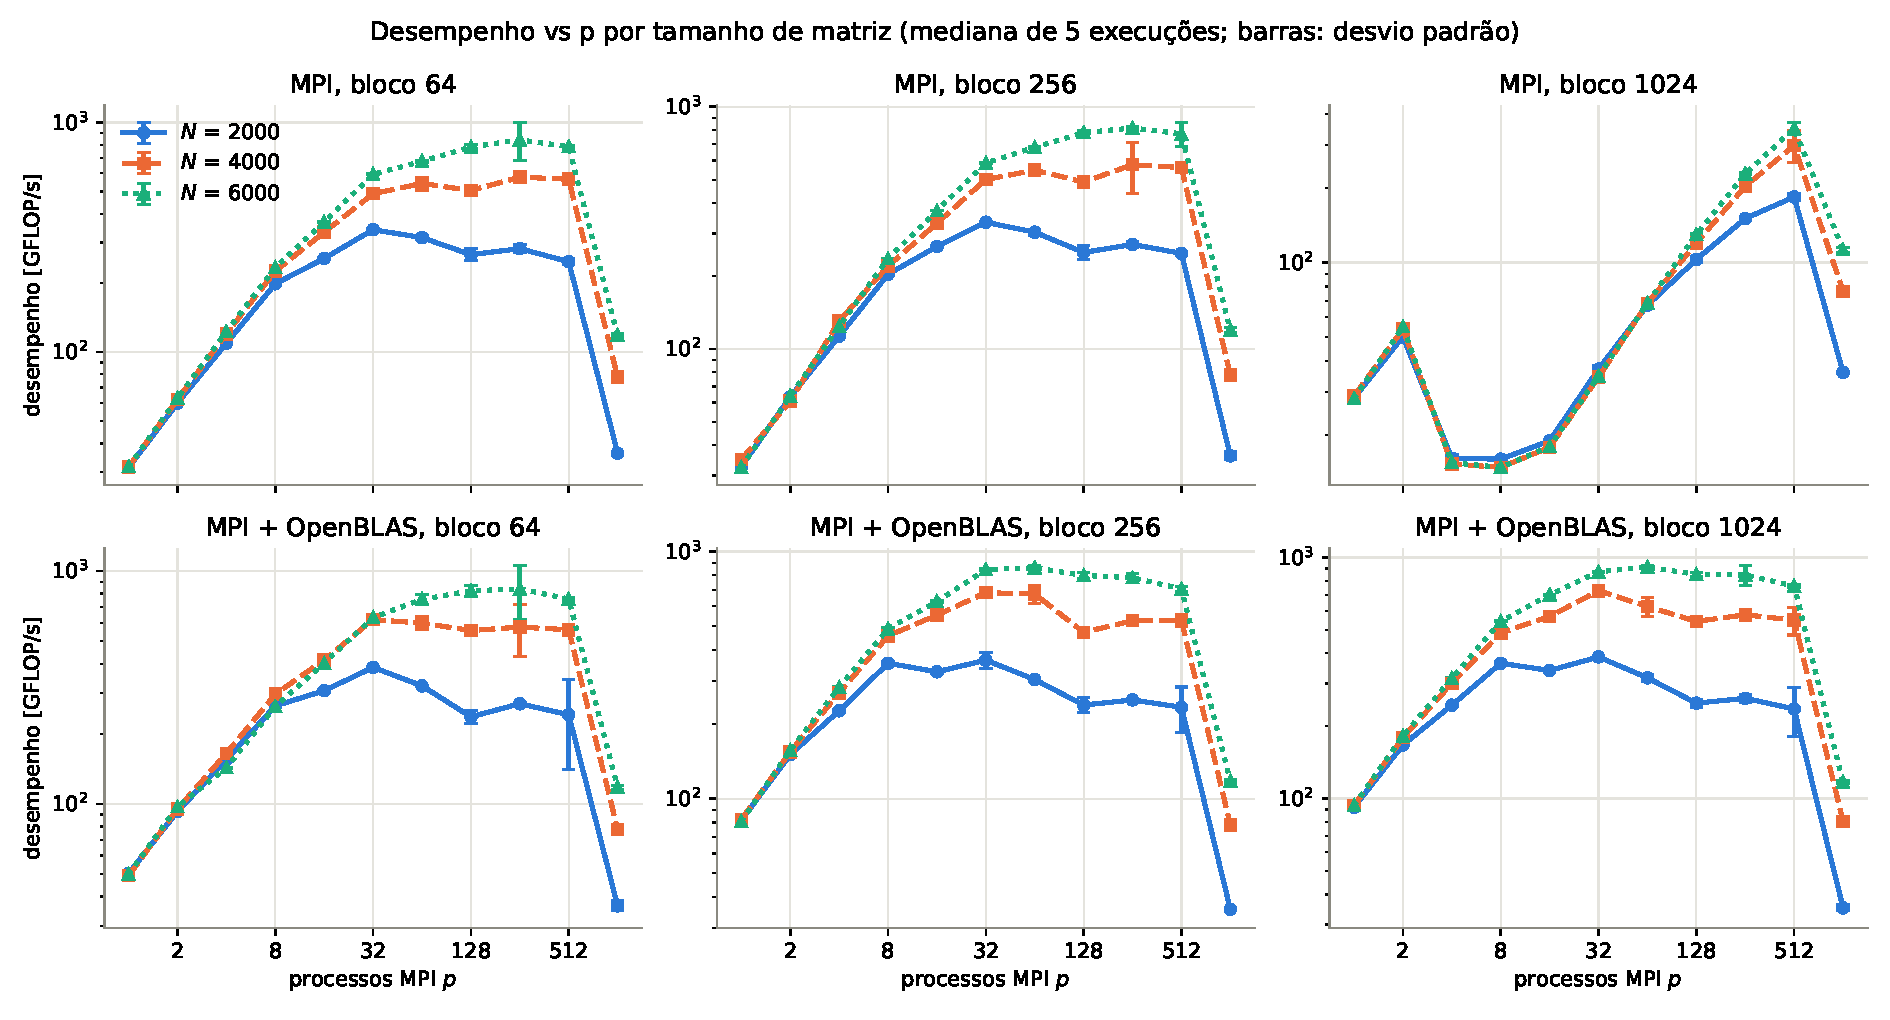
\includegraphics[width=\textwidth]{gflops_tamanhos.pdf}
\vspace{-1ex}
\caption{Desempenho em GFLOP/s, pela Equação~\eqref{eq:gflops}, em função de $p$ para $N=2000$, 4000 e 6000, com um tamanho de bloco por coluna, 64, 256 e 1024, e uma versão por linha, MPI e MPI + OpenBLAS, na escalabilidade forte, com eixos em escala logarítmica. Pontos: mediana de 5 execuções; barras: desvio padrão.}
% fonte: results/metrics.csv, metric=gflops, scaling=strong, nodes=max(1,ceil(p/128)); gerada por scripts/make_figures.py
\label{fig:gflops}
\end{figure}

\section{Análise}
\textbf{Impacto do número de processos MPI.} A Figura~\ref{fig:speedup} e a Tabela~\ref{tab:speedup} mostram o speedup paralelo da Equação~\eqref{eq:sp} em função de $p$. Até $p=8$ o ganho é próximo do ideal para MPI, com $S_8 = 6{,}22$ a 7,28 com bloco 256. Depois a curva se afasta do ideal e atinge um máximo: com bloco 256, $S_p$ da MPI chega a 10,2 em $p=32$ para $N=2000$, a 16,5 em $p=256$ para $N=4000$ e a 25,2 em $p=256$ para $N=6000$; acima disso o tempo volta a subir. MPI + OpenBLAS tem $S_p$ bem menor, com máximo de 4,44, 8,27 e 10,6 com bloco 256, porque o seu kernel é 2,3 a 2,5 vezes mais rápido e a comunicação, idêntica nas duas versões, passa a pesar mais. Em $p=1024$ todas as versões pioram muito: com $N=6000$ e bloco 256 o tempo sobe para 3,61 s na MPI e 3,67 s na MPI + OpenBLAS, contra 0,528 e 0,552 s em $p=256$, como mostra a Tabela~\ref{tab:tempos}.

\begin{figure}[!htb]
\centering
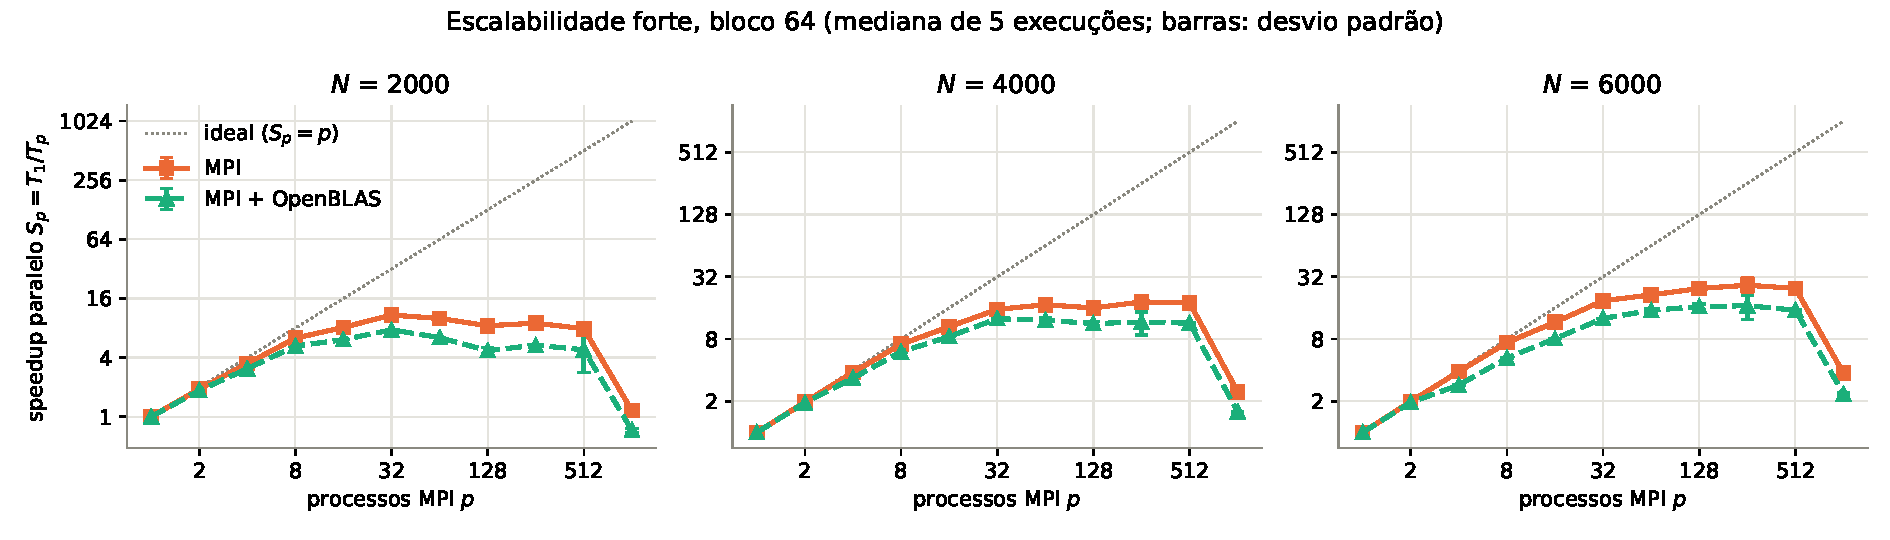
\includegraphics[width=\textwidth]{speedup_parallel_b64.pdf}\\[-0.3ex]
{\small Bloco 64.}\\[0.5ex]
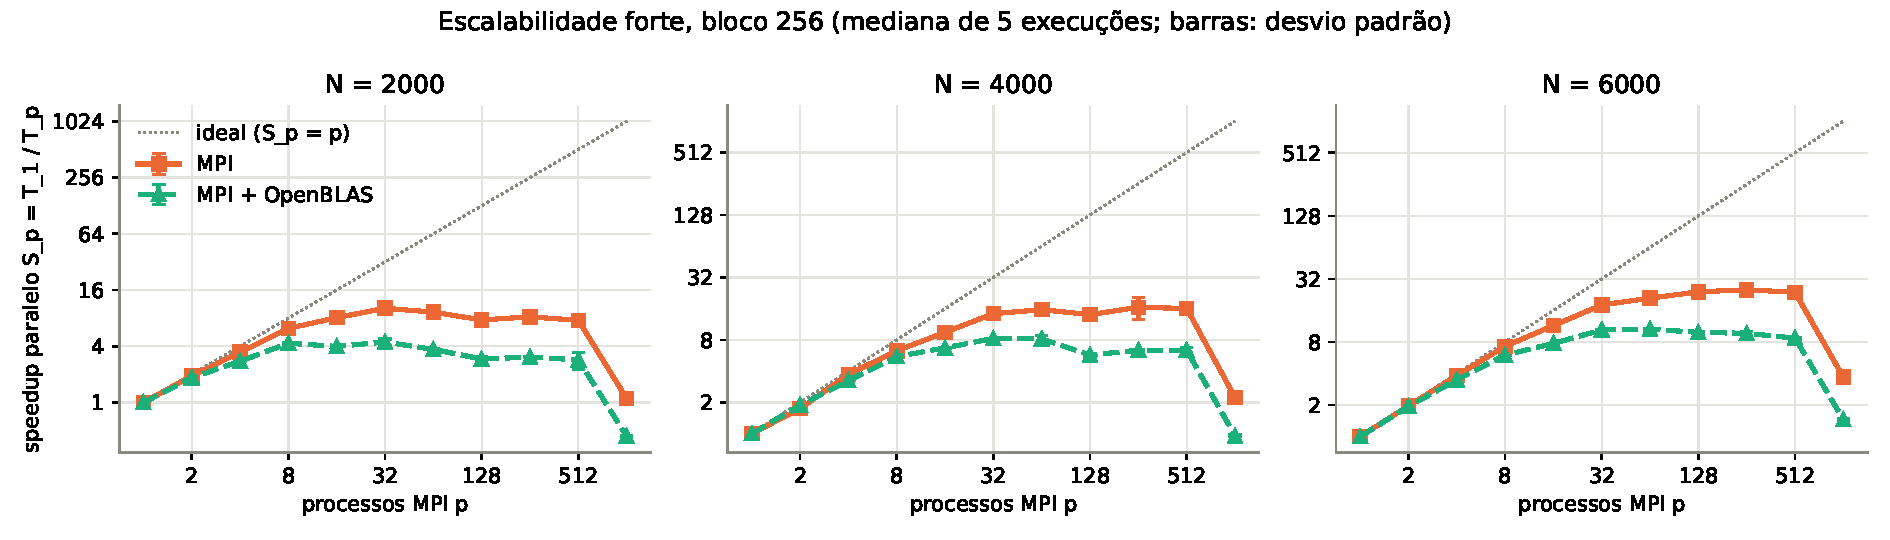
\includegraphics[width=\textwidth]{speedup_parallel_b256.pdf}\\[-0.3ex]
{\small Bloco 256.}\\[0.5ex]
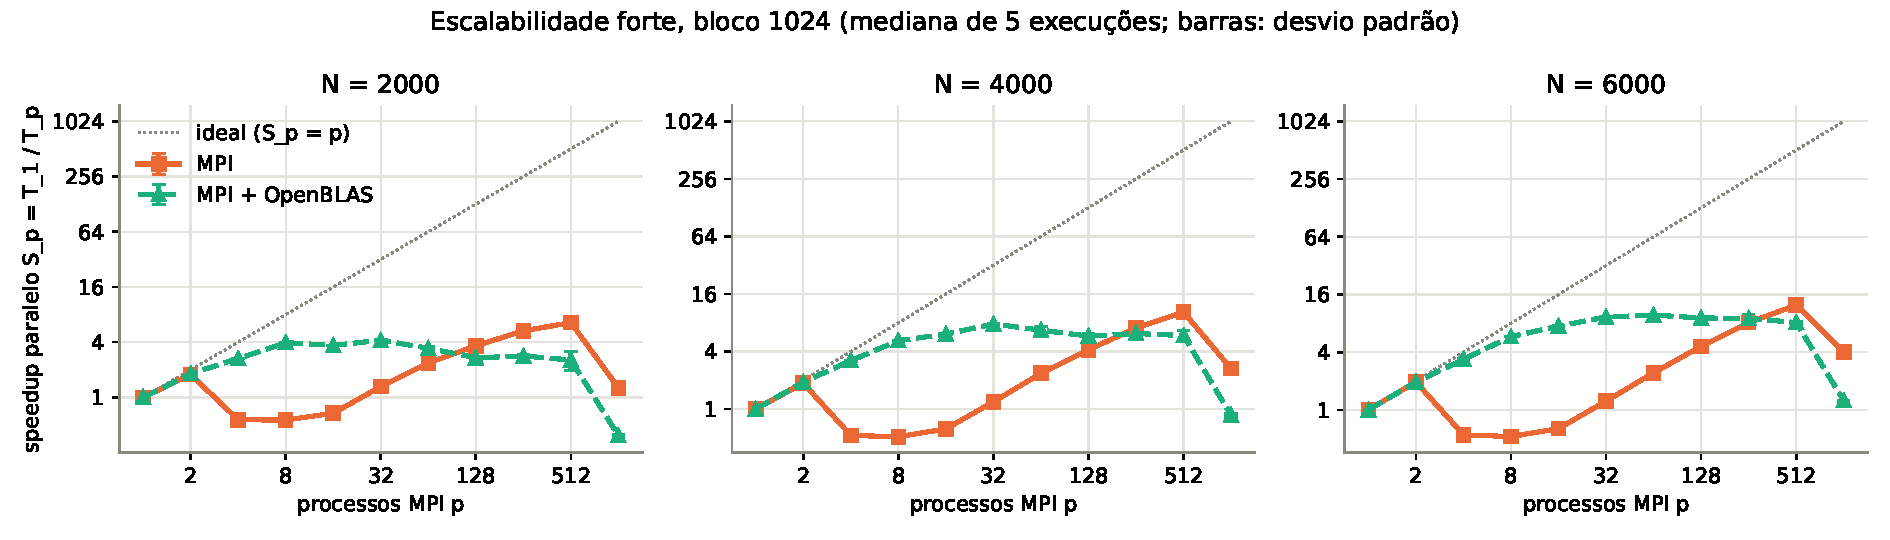
\includegraphics[width=\textwidth]{speedup_parallel_b1024.pdf}\\[-0.3ex]
{\small Bloco 1024.}
\caption{Speedup paralelo $S_p$, pela Equação~\eqref{eq:sp}, em função do número de processos MPI na escalabilidade forte, para $N=2000$, 4000 e 6000, com eixos em escala $\log_2$; de cima para baixo, blocos 64, 256 e 1024. MPI em laranja, MPI + OpenBLAS em verde; pontilhado: ideal $S_p=p$. Pontos: mediana de 5 execuções; barras: desvio padrão. Referência $T_1$: mediana da mesma versão, mesmo $N$ e mesmo bloco, com $p=1$. Com $p\le128$ as execuções ocupam 1 nó; 256, 512 e 1024 processos ocupam 2, 4 e 8 nós.}
% fonte: results/metrics.csv, metric=speedup_parallel, scaling=strong, nodes=max(1,ceil(p/128)); gerada por scripts/make_figures.py
\label{fig:speedup}
\end{figure}

\begin{figure}[!htb]
\centering
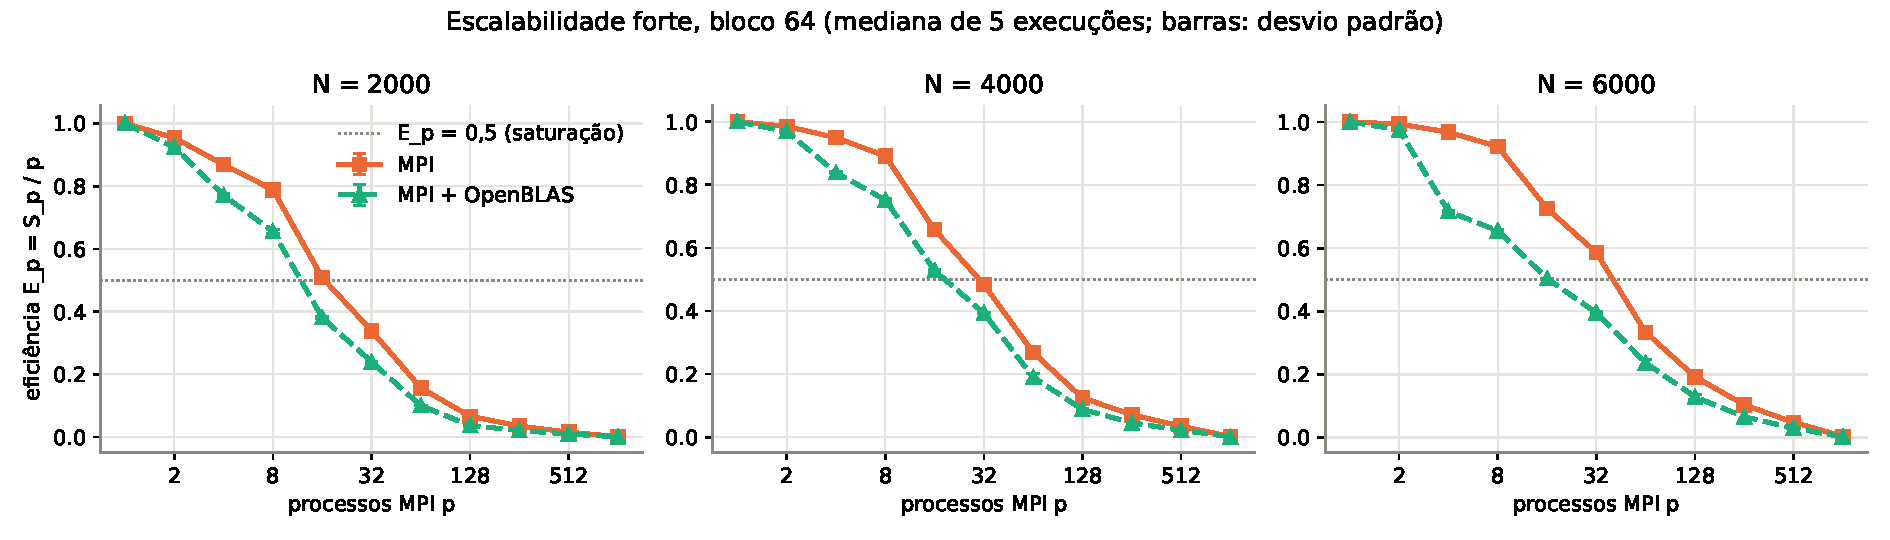
\includegraphics[width=\textwidth]{efficiency_strong_b64.pdf}\\[-0.3ex]
{\small Bloco 64.}\\[0.5ex]
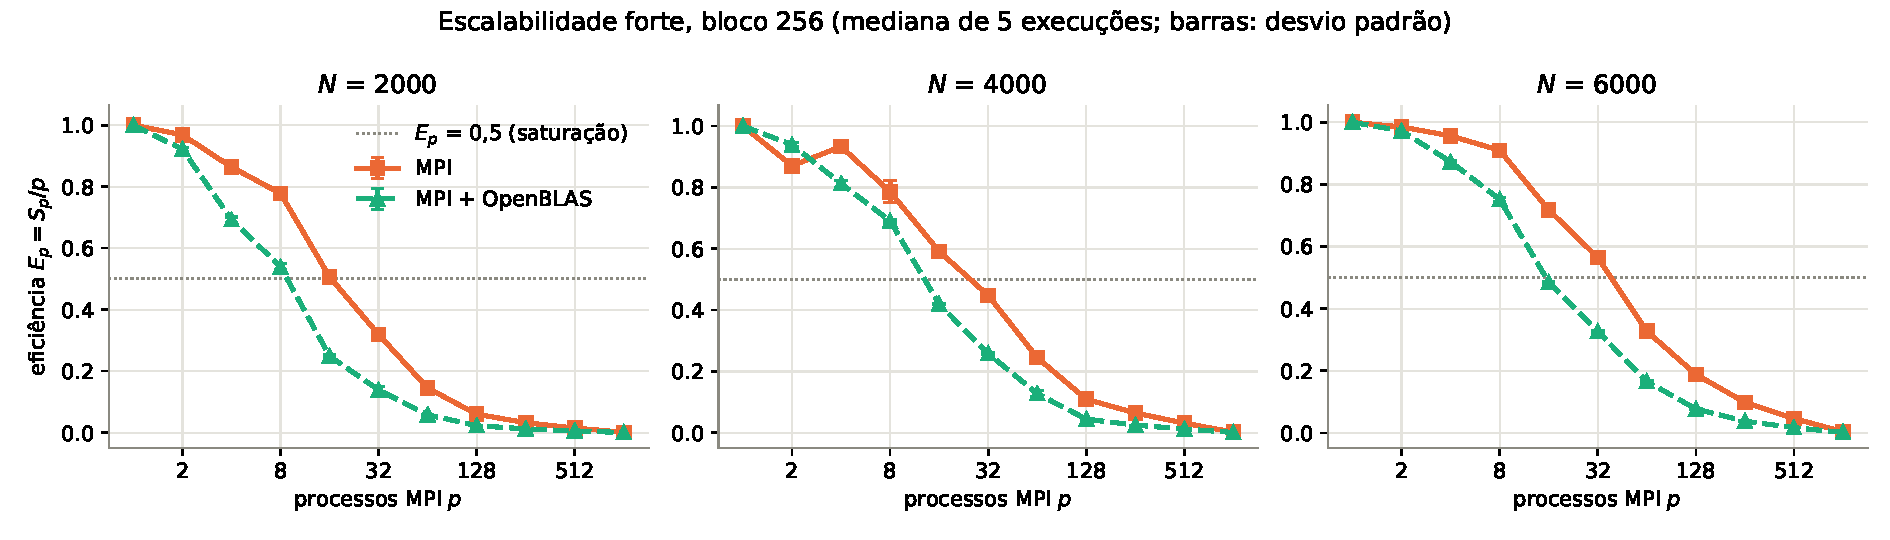
\includegraphics[width=\textwidth]{efficiency_strong_b256.pdf}\\[-0.3ex]
{\small Bloco 256.}\\[0.5ex]
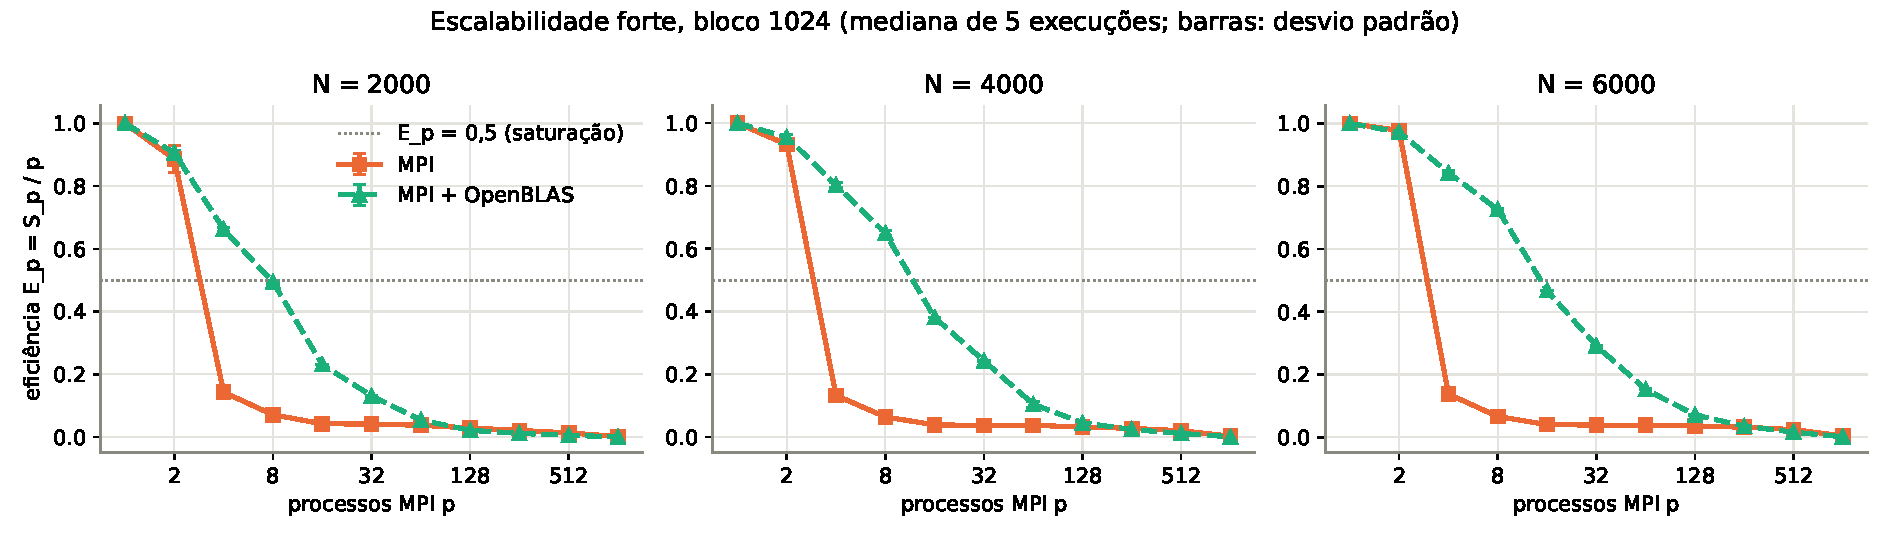
\includegraphics[width=\textwidth]{efficiency_strong_b1024.pdf}\\[-0.3ex]
{\small Bloco 1024.}
\caption{Eficiência forte $E_p$, pela Equação~\eqref{eq:ep}, em função de $p$, para $N=2000$, 4000 e 6000, com eixo $x$ em escala $\log_2$; de cima para baixo, blocos 64, 256 e 1024. Pontilhado: $E_p=0{,}5$, critério de saturação da Equação~\eqref{eq:sat}. Pontos: mediana de 5 execuções; barras: desvio padrão. Mesma referência da Figura~\ref{fig:speedup}.}
% fonte: results/metrics.csv, metric=efficiency_strong, scaling=strong, nodes=max(1,ceil(p/128)); gerada por scripts/make_figures.py
\label{fig:efic}
\end{figure}

\textbf{Escalabilidade forte.} Na escalabilidade forte o tamanho do problema fica fixo e os recursos crescem. A Figura~\ref{fig:efic} mostra a eficiência forte $E_p$ da Equação~\eqref{eq:ep}: ela cai continuamente com $p$ e, com os blocos 64 e 256, fica abaixo de 0,5 a partir de $p=16$ a 64. A Tabela~\ref{tab:sat} dá o ponto de saturação da Equação~\eqref{eq:sat} para cada versão, tamanho e bloco. Para MPI com blocos 64 e 256, $p_{\mathrm{sat}}$ é 32 para $N=2000$ e 4000 e 64 para $N=6000$; para MPI + OpenBLAS é menor, de 8 a 32, pelo motivo já dito: o kernel rápido reduz a parte paralelizável, e o custo fixo da comunicação domina antes. O speedup máximo continua crescendo depois de $p_{\mathrm{sat}}$ em alguns casos, como na MPI com $N=6000$ e $b=256$, que chega a 25,2 em $p=256$, mas com eficiência baixa, $E_{256} = 0{,}0985$.

\begin{table}[!htb]
\centering\footnotesize
\renewcommand{\arraystretch}{1.05}\setlength{\tabcolsep}{4pt}
% fonte: results/saturation.csv (saturation_p, criterion, max_speedup, at_p); desvio de S_p em results/metrics.csv,
% metric=speedup_parallel, scaling=strong, no p de máximo
\begin{tabular}{|l|r|r|r|r|r|r|r|}
\hline
 & & \multicolumn{3}{c|}{\textbf{$p_{\mathrm{sat}}$ e critério}} & \multicolumn{3}{c|}{\textbf{$S_p$ máximo, desvio e $p$}} \\
\textbf{Versão} & \textbf{$N$} & \textbf{$b=64$} & \textbf{$b=256$} & \textbf{$b=1024$} & \textbf{$b=64$} & \textbf{$b=256$} & \textbf{$b=1024$} \\
\hline\hline
MPI & 2000 & 32, $E$ & 32, $E$ & 2, $S$ & \textbf{10,8} (0,13) em 32 & 10,2 (0,062) em 32 & 6,52 (0,20) em 512 \\ \hline
MPI & 4000 & 32, $E$ & 32, $E$ & 2, $S$ & \textbf{18,3} (0,21) em 256 & 16,5 (4,0) em 256 & 10,3 (1,5) em 512 \\ \hline
MPI & 6000 & 64, $E$ & 64, $E$ & 2, $S$ & \textbf{26,5} (4,9) em 256 & 25,2 (0,32) em 256 & 12,4 (0,69) em 512 \\ \hline\hline
MPI + OpenBLAS & 2000 & 16, $E$ & 8, $S$ & 8, $E$ & \textbf{7,67} (0,056) em 32 & 4,44 (0,34) em 32 & 4,20 (0,021) em 32 \\ \hline
MPI + OpenBLAS & 4000 & 32, $E$ & 16, $E$ & 16, $E$ & \textbf{12,6} (0,055) em 32 & 8,27 (0,058) em 32 & 7,77 (0,046) em 32 \\ \hline
MPI + OpenBLAS & 6000 & 32, $E$ & 16, $E$ & 16, $E$ & \textbf{16,8} (4,3) em 256 & 10,6 (0,21) em 64 & 9,76 (0,12) em 64 \\ \hline
\end{tabular}
\caption{Ponto de saturação $p_{\mathrm{sat}}$ da Equação~\eqref{eq:sat}: menor $p$ com $E_p<0{,}5$, critério $E$, ou com $S_p$ do $p$ seguinte menor ou igual a $S_p$, critério $S$. À direita, o maior $S_p$ da série forte, com a mediana, o desvio padrão e o $p$ onde ocorre. Referência: mesma versão, $N$ e $b$, com $p=1$. Os desvios de 4,0 a 4,9 vêm de uma execução lenta isolada no job multinó. Em negrito: maior $S_p$ de cada linha.}
\label{tab:sat}
\end{table}

\textbf{Impacto do número de núcleos.} Como há 1 processo por núcleo, o número de núcleos ocupados é igual a $p$; os núcleos reservados são sempre nós inteiros, de 128 núcleos. Em 1 nó, ocupar a segunda metade dos núcleos rende pouco: de $p=64$ para $p=128$, MPI com $N=6000$ e bloco 256 passa de 0,635 para 0,552 s, e MPI + OpenBLAS com bloco 1024 piora, de 0,473 para 0,508 s. Na MPI o cálculo ainda cai, de 0,317 para 0,169 s, mas a distribuição cresce, de 0,311 para 0,381 s, e os 128 ranks disputam a banda de memória do nó. A varredura de nós da Tabela~\ref{tab:nos} confirma que a ocupação por nó importa: os mesmos 128 processos espalhados em 2 nós, com 64 núcleos ocupados em cada, são 1,22 a 1,41 vezes mais rápidos que em 1 nó cheio com bloco 256.
% fonte: results/metrics.csv (time_total_s, time_compute_s, time_distribution_s; N=6000, strong, p=64 e 128); A3 4.1 e quebra N=6000

\textbf{Impacto do número de nós.} Na série forte, $p$ e o número de nós crescem juntos, com 128 processos por nó. Passar de 1 para 2 nós, isto é, de $p=128$ para 256, ainda melhora um pouco a MPI com $N=4000$ e 6000, de 0,552 para 0,528 s com $N=6000$ e bloco 256. Já 4 nós, com $p=512$, pioram, e 8 nós, com $p=1024$, elevam o tempo para 3,61 s, contra 0,552 s em $p=128$: a distribuição sozinha leva 3,56 s com $N=6000$, como mostra a Tabela~\ref{tab:fases}. Para separar o efeito dos nós do efeito dos processos, a varredura fixa $p=128$ e o espalha em 1, 2, 4 e 8 nós, na Figura~\ref{fig:nos} e na Tabela~\ref{tab:nos}. Sair do nó não custa: 2 e 8 nós são mais rápidos que 1 nó, com razão de 1,20 a 1,52 para blocos 64 e 256, pois cada rank ganha banda de memória e cache e a comunicação intranó do \texttt{Bcast} disputa menos recursos. Com 4 nós a razão fica só em 1,04 a 1,19, abaixo de 2 e de 8 nós; a medição não explica essa diferença, e os conjuntos de hosts mudam entre 2, 4 e 8 nós, como discutem as Limitações. A MPI com bloco 1024, dominada pelo cálculo, quase não muda, com razão de 1,01 a 1,13.

\begin{table}[!htb]
\centering\footnotesize
\renewcommand{\arraystretch}{1.05}\setlength{\tabcolsep}{2.5pt}
% fonte: results/node_sweep.csv (median_total_s, std_total_s, node_ratio), p=128; 1 nó do job 1034860 (par128, adano35),
% 2/4/8 nós do job 1034865 (paralela)
\begin{tabular}{|l|r|r|r|r|r|r|r|r|r|}
\hline
\textbf{Versão} & \textbf{$b$} & \textbf{$N$} & \textbf{1 nó, 128/nó} & \textbf{2 nós, 64/nó} & \textbf{4 nós, 32/nó} & \textbf{8 nós, 16/nó} & \textbf{Razão 2} & \textbf{Razão 4} & \textbf{Razão 8} \\
\hline\hline
MPI & 256 & 2000 & 0,0639 (0,0045) & 0,0455 (0,0011) & 0,0567 (0,0032) & \textbf{0,0446} (0,00027) & 1,41 & 1,13 & \textbf{1,43} \\ \hline
MPI & 256 & 4000 & 0,262 (0,011) & \textbf{0,193} (0,0013) & 0,223 (0,0036) & 0,193 (0,0010) & \textbf{1,36} & 1,18 & 1,35 \\ \hline
MPI & 256 & 6000 & 0,552 (0,014) & 0,454 (0,0014) & 0,512 (0,0069) & \textbf{0,442} (0,0019) & 1,22 & 1,08 & \textbf{1,25} \\ \hline\hline
MPI + OpenBLAS & 256 & 2000 & 0,0669 (0,0054) & 0,0490 (0,00058) & 0,0608 (0,0025) & \textbf{0,0483} (0,00063) & 1,37 & 1,10 & \textbf{1,39} \\ \hline
MPI + OpenBLAS & 256 & 4000 & 0,272 (0,011) & \textbf{0,201} (0,0018) & 0,237 (0,0031) & 0,209 (0,00071) & \textbf{1,36} & 1,15 & 1,30 \\ \hline
MPI + OpenBLAS & 256 & 6000 & 0,541 (0,016) & \textbf{0,435} (0,0048) & 0,512 (0,0069) & 0,450 (0,0015) & \textbf{1,24} & 1,06 & 1,20 \\ \hline\hline
MPI & 1024 & 6000 & 3,33 (0,029) & 3,25 (0,26) & 3,29 (0,090) & \textbf{3,23} (0,0035) & 1,03 & 1,01 & \textbf{1,03} \\ \hline
\end{tabular}
\caption{Varredura de nós com $p=128$ fixo: tempo total em segundos, com mediana e desvio padrão de 5 execuções, e razão $T(1\text{ nó})/T(k\text{ nós})$ das medianas; uma razão acima de 1 indica execução mais rápida em $k$ nós. Em negrito: menor tempo de cada linha e a razão correspondente.}
\label{tab:nos}
\end{table}

\begin{figure}[!htb]
\centering
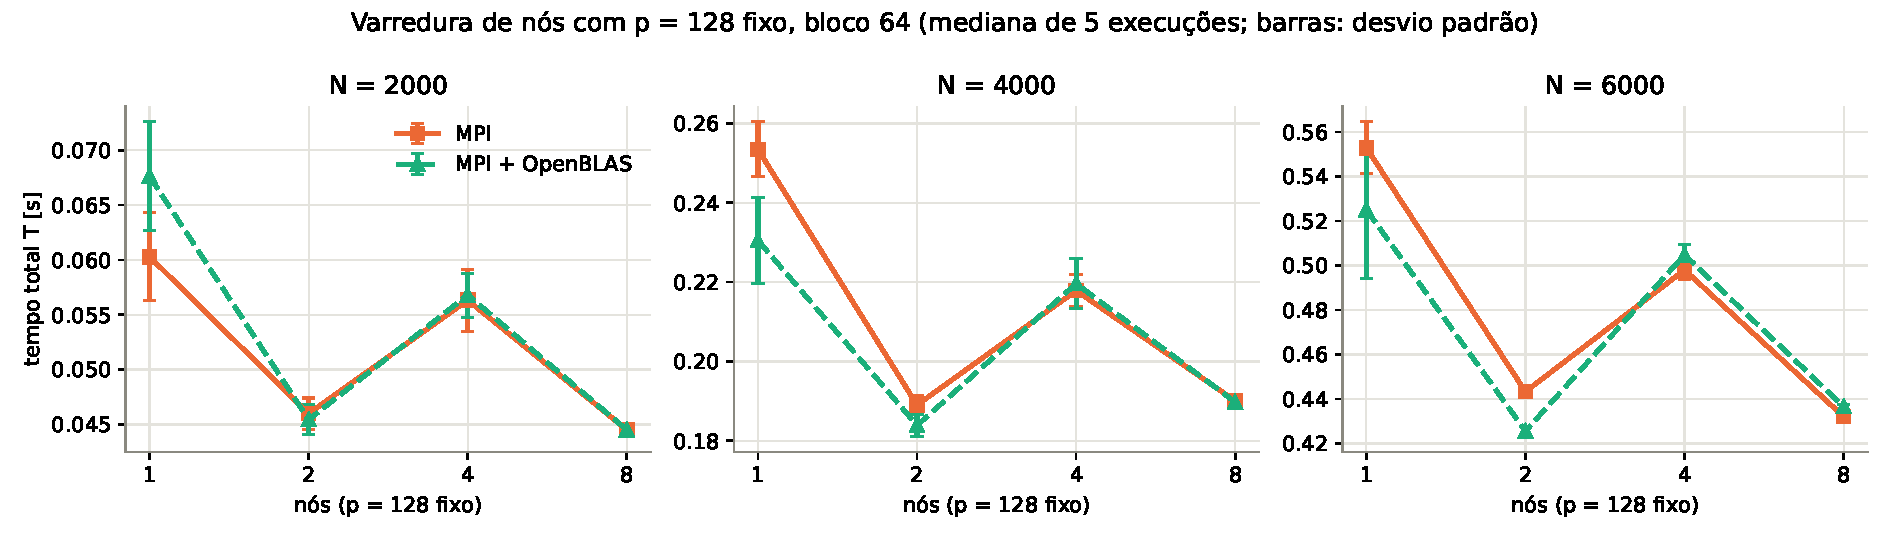
\includegraphics[width=\textwidth]{node_sweep_b64.pdf}\\[-0.3ex]
{\small Bloco 64.}\\[0.5ex]
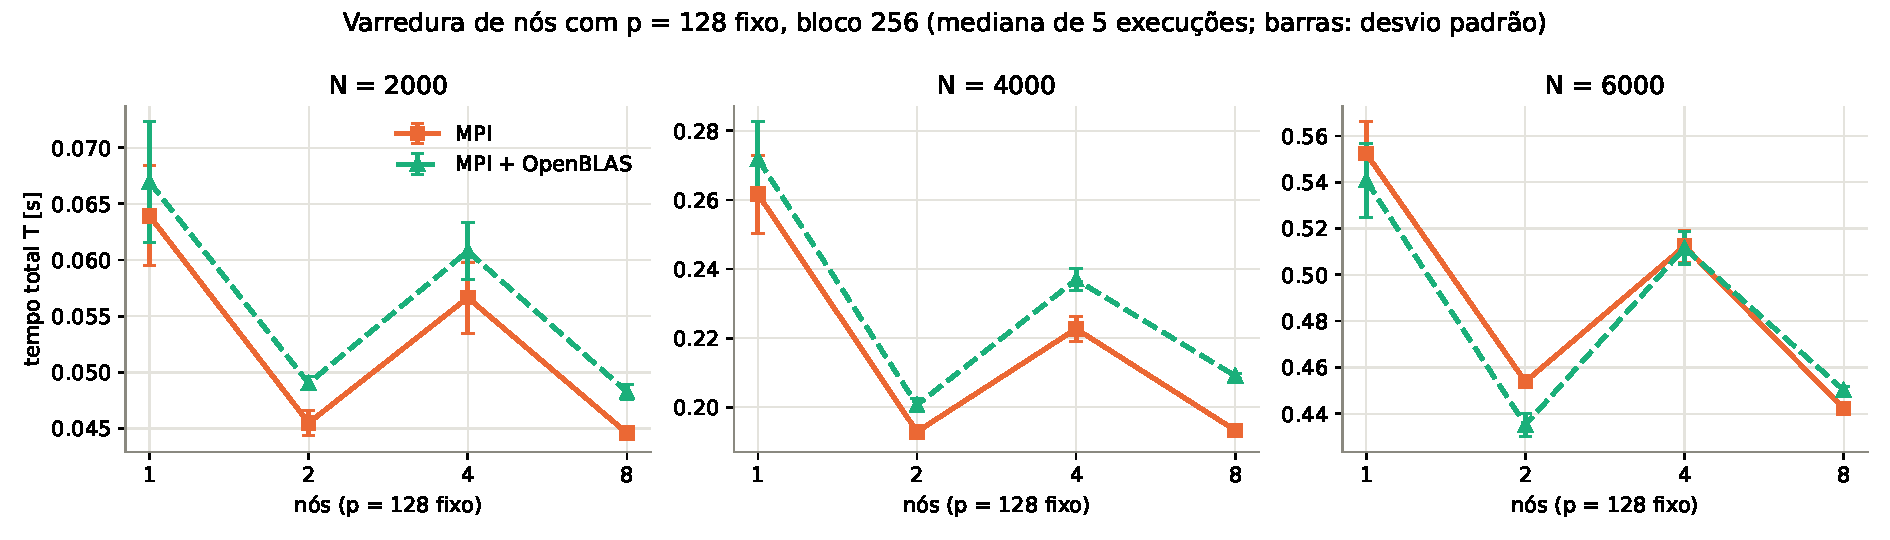
\includegraphics[width=\textwidth]{node_sweep_b256.pdf}\\[-0.3ex]
{\small Bloco 256.}\\[0.5ex]
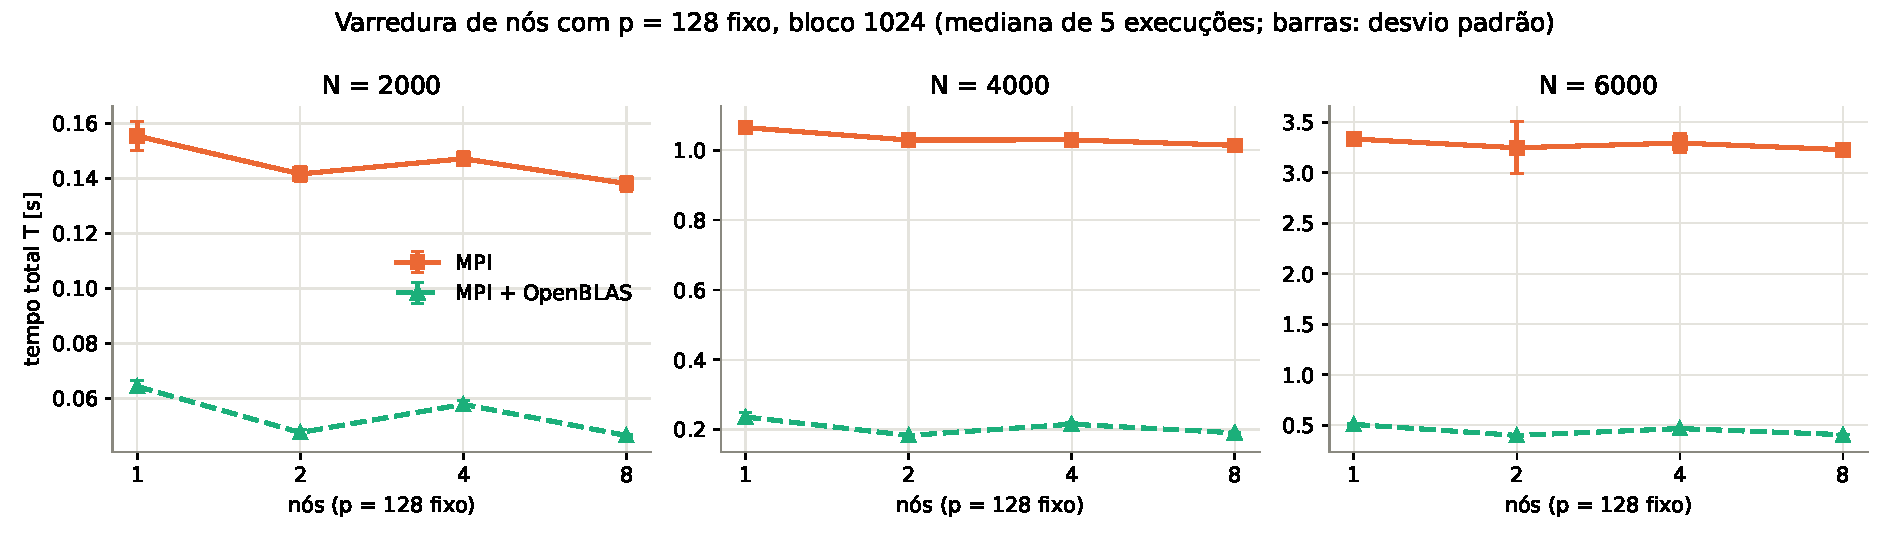
\includegraphics[width=\textwidth]{node_sweep_b1024.pdf}\\[-0.3ex]
{\small Bloco 1024.}
\caption{Tempo total com $p=128$ fixo distribuído em 1, 2, 4 e 8 nós, com 128, 64, 32 e 16 processos por nó, para $N=2000$, 4000 e 6000; de cima para baixo, blocos 64, 256 e 1024. Pontos: mediana de 5 execuções; barras: desvio padrão. O ponto de 1 nó vem do job \texttt{par128}; os demais, do job 1034865 na fila \texttt{paralela}.}
% fonte: results/node_sweep.csv (median_total_s, std_total_s), filtro block_size; gerada por scripts/make_figures.py
\label{fig:nos}
\end{figure}

\textbf{Influência do tamanho das matrizes.} O trabalho cresce com $2N^3$, 27 vezes de $N=2000$ para $N=6000$, enquanto o volume de $B$ difundido a cada rank cresce com $N^2$, só 9 vezes; a razão entre cálculo e comunicação cresce, portanto, com $N$. Por isso matrizes maiores escalam mais: o $S_p$ máximo da MPI com bloco 256 vai de 10,2 com $N=2000$ para 16,5 com 4000 e 25,2 com 6000, $p_{\mathrm{sat}}$ passa de 32 para 64, e o GFLOP/s máximo vai de 341 para 840, como mostra a Figura~\ref{fig:gflops}. Com $N=2000$ o tempo total é de dezenas de milissegundos a partir de $p=8$, e a comunicação passa a dominar já em $p=16$, com $f_{\mathrm{com}}=0{,}41$ na MPI com bloco 64. Na Serial, o GFLOP/s quase não depende de $N$: 33,3, 35,5 e 33,1 com bloco 256.

\begin{table}[!htb]
\centering\footnotesize
\renewcommand{\arraystretch}{1.05}\setlength{\tabcolsep}{3.5pt}
% fonte: results/metrics.csv, metric=time_total_s, scaling=strong, p in {1, 8}, nodes=1; value (mediana) e std
\begin{tabular}{|r|l|r|r|r|r|r|r|}
\hline
 & & \multicolumn{3}{c|}{\textbf{$p=1$}} & \multicolumn{3}{c|}{\textbf{$p=8$}} \\
\textbf{$N$} & \textbf{Versão} & \textbf{$b=64$} & \textbf{$b=256$} & \textbf{$b=1024$} & \textbf{$b=64$} & \textbf{$b=256$} & \textbf{$b=1024$} \\
\hline\hline
2000 & Serial & 0,513 (0,0024) & \textbf{0,480} (0,0035) & 0,562 (0,00033) &  &  &  \\ \hline
2000 & MPI & 0,509 (0,0021) & \textbf{0,490} (0,0065) & 0,566 (0,00057) & 0,0807 (0,00063) & \textbf{0,0787} (0,00089) & 1,00 (0,016) \\ \hline
2000 & MPI + OpenBLAS & 0,318 (0,0022) & 0,196 (0,00056) & \textbf{0,174} (0,0012) & 0,0607 (0,00057) & 0,0454 (0,00081) & \textbf{0,0440} (0,00050) \\ \hline\hline
4000 & Serial & 4,06 (0,0090) & \textbf{3,60} (0,029) & 4,41 (0,0042) &  &  &  \\ \hline
4000 & MPI & 4,05 (0,0051) & \textbf{3,67} (0,0073) & 4,44 (0,0036) & \textbf{0,568} (0,0011) & 0,583 (0,025) & 8,64 (0,013) \\ \hline
4000 & MPI + OpenBLAS & 2,60 (0,00058) & 1,55 (0,026) & \textbf{1,37} (0,0082) & 0,433 (0,0019) & 0,281 (0,0016) & \textbf{0,263} (0,0034) \\ \hline\hline
6000 & Serial & 13,6 (0,015) & \textbf{13,0} (0,042) & 15,3 (0,011) &  &  &  \\ \hline
6000 & MPI & 13,6 (0,015) & \textbf{13,3} (0,025) & 15,4 (0,026) & 1,85 (0,0025) & \textbf{1,83} (0,0043) & 29,1 (0,15) \\ \hline
6000 & MPI + OpenBLAS & 8,66 (0,019) & 5,34 (0,020) & \textbf{4,62} (0,032) & 1,65 (0,0061) & 0,889 (0,0080) & \textbf{0,795} (0,0046) \\ \hline
\end{tabular}
\caption{Efeito do tamanho de bloco $b$: tempo total em segundos, com mediana e desvio padrão de 5 execuções, com $p=1$ e $p=8$ em 1 nó. A Serial só existe com $p=1$. Em negrito: melhor bloco de cada linha, isto é, o de menor tempo, para cada $p$.}
\label{tab:blocos}
\end{table}

\textbf{Influência do tamanho de bloco.} A Tabela~\ref{tab:blocos} e a Figura~\ref{fig:tempo} comparam os blocos. Na Serial e na MPI com $p=1$ o melhor bloco é 256: com $N=6000$, a Serial leva 13,0 s com $b=256$, 13,6 s com $b=64$ e 15,3 s com $b=1024$. O ladrilho de 256, com 256 KiB, cabe no L2 de 512 KiB; o de 64 tem laços internos curtos; e o de 1024, com 4 MiB, não cabe no L2. A MPI com $b=1024$ degrada muito de $p=4$ a $p=32$: com $N=6000$, leva 27,9 s em $p=4$, contra 7,85 s em $p=2$ e 3,48 s com $b=256$ em $p=4$. O tempo volta a cair quando $p$ cresce e a faixa local encolhe, chegando a 3,33 s em $p=128$. Uma hipótese, não verificada por falta de contadores de hardware, é a disputa pelo L3 de 16 MiB compartilhado por CCX quando vários ranks, cada um com ladrilhos de 4 MiB, ocupam o mesmo CCX. Na MPI + OpenBLAS ocorre o contrário: blocos maiores são melhores com $p$ pequeno, com 8,66, 5,34 e 4,62 s para $b=64$, 256 e 1024 com $N=6000$ e $p=1$, porque cada ladrilho é uma chamada \texttt{sgemm}, e ladrilhos maiores amortizam o custo de chamada e deixam o OpenBLAS usar o seu próprio bloqueio interno. Com $p\ge128$, quando a comunicação domina, a diferença entre blocos na MPI + OpenBLAS fica entre 5 e 18\,\%.
% fonte: results/metrics.csv time_total_s strong; A3 4.5 (spread 5 a 18 % para p >= 128)

\begin{figure}[!htb]
\centering
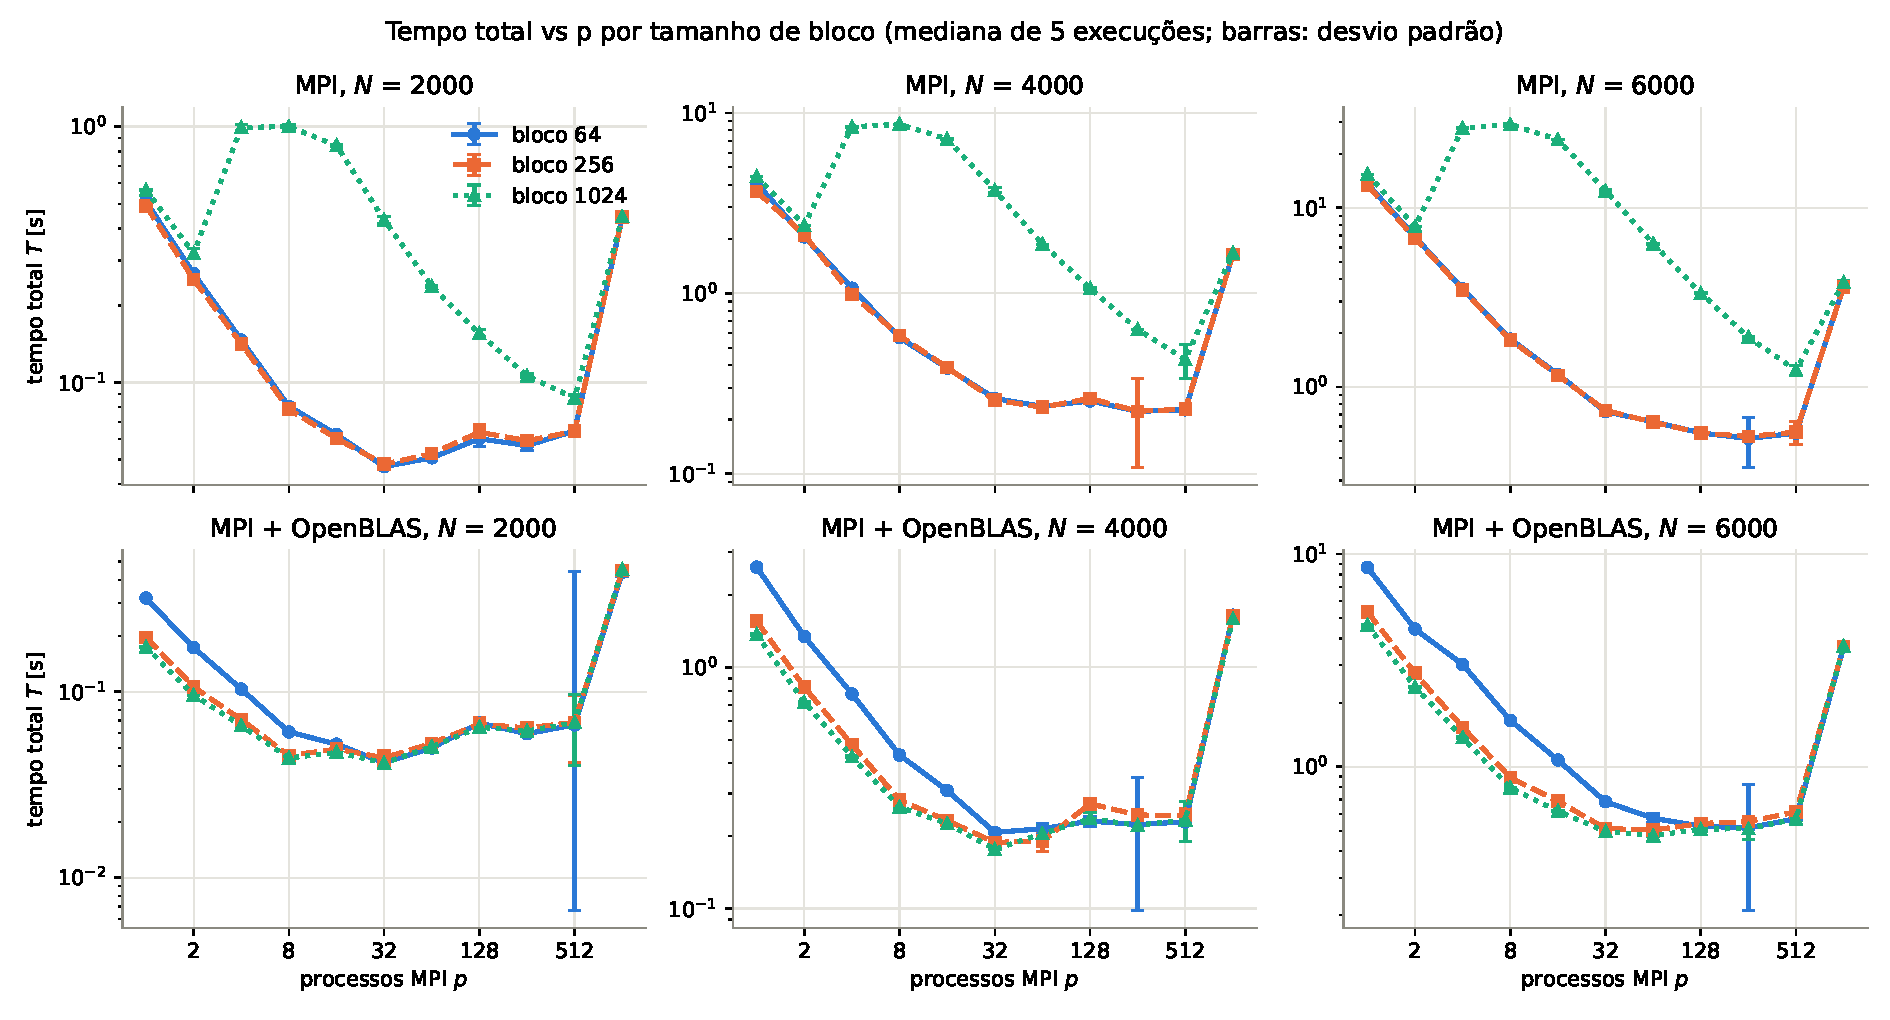
\includegraphics[width=\textwidth]{tempo_blocos.pdf}
\vspace{-1ex}
\caption{Tempo total em função do número de processos MPI para blocos 64, 256 e 1024, com a MPI na linha de cima e a MPI + OpenBLAS na de baixo, para $N=2000$, 4000 e 6000, na escalabilidade forte, com eixos em escala logarítmica. Pontos: mediana de 5 execuções; barras: desvio padrão. As barras longas em $p=256$ e 512 vêm de uma execução lenta isolada.}
% fonte: results/metrics.csv, metric=time_total_s, scaling=strong, nodes=max(1,ceil(p/128)); gerada por scripts/make_figures.py
\label{fig:tempo}
\end{figure}

\textbf{Escalabilidade fraca.} Na escalabilidade fraca o tamanho cresce com $p$ para manter aproximadamente constante o trabalho por processo. Como o custo é $2N^3$, as razões de trabalho entre $N=2000$, 4000 e 6000 são $1:8:27$, e os pares escolhidos dão exatamente o mesmo trabalho por processo:
\begin{equation}\label{eq:fraca}
\frac{2\cdot 2000^3}{1} = \frac{2\cdot 4000^3}{8} = \frac{2\cdot 6000^3}{27} = 1{,}6\cdot 10^{10}\ \text{FLOP} = 16\ \text{GFLOP},
\end{equation}
em que cada numerador é o número de operações $2N^3$ do produto e cada denominador o número de processos $p$ do par. A Tabela~\ref{tab:fraca} e a Figura~\ref{fig:fraca} mostram a eficiência fraca da Equação~\eqref{eq:ew}. Com bloco 64, a MPI mantém $E_w = 0{,}893$ em $p=8$ e cai para 0,591 em $p=27$; a MPI + OpenBLAS cai mais, para 0,738 e 0,385 com $b=64$ e para 0,665 e 0,316 com $b=1024$. Dois efeitos se somam. A distribuição cresce, pois cada rank recebe $B$ inteira, com $N^2$ elementos: com bloco 64, ela leva 0,046 s em $(4000,8)$ e 0,257 s em $(6000,27)$, e $f_{\mathrm{com}}$ vai de 0,088 a 0,32 na MPI. E o próprio cálculo por processo fica mais lento, embora o trabalho seja o mesmo: na MPI com bloco 64, de 0,508 s para 0,518 e 0,588 s, e na MPI + OpenBLAS com bloco 1024, de 0,174 s para 0,208 e 0,257 s, o que indica disputa pela memória e pelo L3 compartilhados e uma matriz $B$ maior. A MPI com bloco 1024 tem $E_w$ de 0,066 e 0,040, o mesmo colapso de $b=1024$ com $4\le p\le32$ visto na escalabilidade forte.
% fonte: results/metrics.csv scaling=weak (time_total_s, time_distribution_s, time_compute_s, efficiency_weak, comm_fraction)

\begin{table}[!htb]
\centering\footnotesize
\renewcommand{\arraystretch}{1.05}\setlength{\tabcolsep}{4pt}
% fonte: results/metrics.csv, scaling=weak, metric in {time_total_s, efficiency_weak, comm_fraction}; value (mediana) e std;
% referência de E_w na coluna reference, por exemplo T_mpi(N=2000, b=64, p=1) = 0.50799 s
\begin{tabular}{|l|r|r|r|r|r|r|r|r|}
\hline
 & & \textbf{$(2000,1)$} & \multicolumn{3}{c|}{\textbf{$(4000,8)$}} & \multicolumn{3}{c|}{\textbf{$(6000,27)$}} \\
\textbf{Versão} & \textbf{$b$} & \textbf{$T$ [s]} & \textbf{$T$ [s]} & \textbf{$E_w$} & \textbf{$f_{\mathrm{com}}$} & \textbf{$T$ [s]} & \textbf{$E_w$} & \textbf{$f_{\mathrm{com}}$} \\
\hline\hline
MPI & 64 & 0,508 (0,0038) & \textbf{0,569} (0,0014) & \textbf{0,893} (0,0023) & 0,088 & 0,860 (0,0027) & \textbf{0,591} (0,0019) & 0,32 \\ \hline
MPI & 256 & \textbf{0,488} (0,0029) & 0,582 (0,0038) & 0,839 (0,0055) & 0,086 & \textbf{0,848} (0,014) & 0,576 (0,0091) & 0,33 \\ \hline
MPI & 1024 & 0,566 (0,0012) & 8,58 (0,034) & 0,0660 (0,00026) & 0,0059 & 14,0 (0,12) & 0,0404 (0,00036) & 0,022 \\ \hline\hline
MPI + OpenBLAS & 64 & 0,319 (0,0022) & 0,432 (0,0019) & \textbf{0,738} (0,0032) & 0,12 & 0,828 (0,0035) & \textbf{0,385} (0,0016) & 0,34 \\ \hline
MPI + OpenBLAS & 256 & 0,196 (0,00044) & 0,284 (0,0012) & 0,689 (0,0030) & 0,18 & 0,566 (0,0053) & 0,346 (0,0032) & 0,52 \\ \hline
MPI + OpenBLAS & 1024 & \textbf{0,174} (0,0011) & \textbf{0,261} (0,0014) & 0,665 (0,0035) & 0,20 & \textbf{0,550} (0,0023) & 0,316 (0,0013) & 0,53 \\ \hline
\end{tabular}
\caption{Escalabilidade fraca em 1 nó, com os pares $(N,p)$ da Equação~\eqref{eq:fraca}, de 16 GFLOP por processo: mediana e desvio padrão de 5 execuções. $E_w$ pela Equação~\eqref{eq:ew}, com referência na mesma versão e bloco, $N=2000$ e $p=1$, que é a coluna $(2000,1)$, onde $E_w=1$. $f_{\mathrm{com}}$ pela Equação~\eqref{eq:fcom}, mediana. Em negrito: melhor bloco de cada versão em cada coluna, isto é, menor $T$ e maior $E_w$.}
\label{tab:fraca}
\end{table}

\begin{figure}[!htb]
\centering
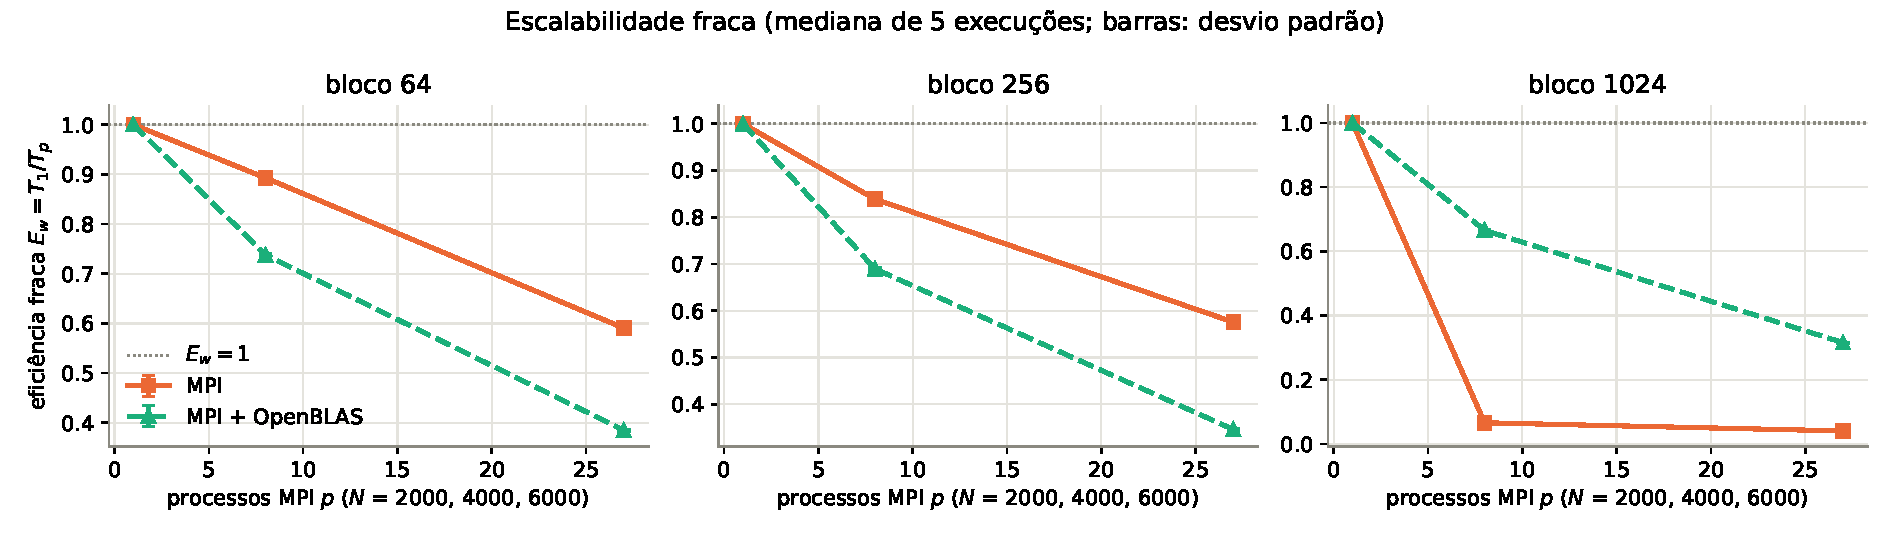
\includegraphics[width=\textwidth]{efficiency_weak.pdf}
\vspace{-1ex}
\caption{Eficiência fraca $E_w$, pela Equação~\eqref{eq:ew}, com trabalho por processo constante, $N=2000$, 4000 e 6000 com $p=1$, 8 e 27, para blocos 64, 256 e 1024, um por painel. MPI em laranja, MPI + OpenBLAS em verde; pontilhado: $E_w=1$. Pontos: mediana de 5 execuções; barras: desvio padrão, menores que os marcadores. Referência: mesma versão e bloco com $N=2000$ e $p=1$.}
% fonte: results/metrics.csv, metric=efficiency_weak, scaling=weak; gerada por scripts/make_figures.py
\label{fig:fraca}
\end{figure}

\textbf{Decomposição do tempo.} A Tabela~\ref{tab:fases} e as Figuras~\ref{fig:fases}, \ref{fig:fases2} e~\ref{fig:fases3} separam distribuição, cálculo e coleta, definidos na Equação~\eqref{eq:fases}. O cálculo cai aproximadamente com $1/p$, e a distribuição cresce com $p$. Na MPI com $N=6000$ e bloco 256 a distribuição alcança o cálculo em $p=64$, com 0,311 contra 0,317 s, e o supera em $p=128$, com 0,381 contra 0,169 s; na MPI + OpenBLAS, cujo cálculo é mais curto, isso já ocorre em $p=32$, com 0,248 contra 0,233 s. Com $N=2000$ o cruzamento ocorre antes, entre $p=8$ e 32. A fração $f_{\mathrm{com}}$ da Equação~\eqref{eq:fcom} acompanha a queda de $E_p$: na MPI com $N=6000$ e bloco 256 ela vai de 0,063 em $p=8$, onde $E_p=0{,}91$, a 0,33 em $p=32$, onde $E_p=0{,}56$, a 0,69 em $p=128$, onde $E_p=0{,}19$, e a 0,98 em $p=1024$. Os máximos por fase não somam o total: pela Equação~\eqref{eq:max}, cada coluna é um máximo independente entre os ranks, e a coleta medida no rank 0 inclui a espera pelo rank mais lento. Por exemplo, na escalabilidade fraca da MPI com $N=6000$ e bloco 1024, o cálculo leva 13,69 s e a coleta 12,82 s, para um total de 14,01 s.
% fonte: results/metrics.csv, metric in {time_distribution_s, time_compute_s, time_gather_s, time_total_s, comm_fraction}; A3 quebra N=2000 e N=6000

\begin{table}[!htb]
\centering\scriptsize
\renewcommand{\arraystretch}{1.05}\setlength{\tabcolsep}{3.5pt}
% fonte: results/metrics.csv, N=6000, scaling=strong, nodes=max(1,ceil(p/128)), MPI b=256 e MPI+OpenBLAS b=1024,
% metric in {time_total_s, time_distribution_s, time_compute_s, time_gather_s, comm_fraction}; value (mediana) e std
\begin{tabular}{|l|r|r|r|r|r|r|r|}
\hline
\textbf{Versão} & \textbf{$p$} & \textbf{Nós} & \textbf{Total [s]} & \textbf{Distribuição [s]} & \textbf{Cálculo [s]} & \textbf{Coleta [s]} & \textbf{$f_{\mathrm{com}}$} \\
\hline\hline
MPI, $b=256$ & 1 & 1 & 13,3 (0,025) & $1{,}9\cdot10^{-6}$ ($3{,}5\cdot10^{-7}$) & 13,3 (0,025) & $9{,}7\cdot10^{-6}$ ($1{,}1\cdot10^{-6}$) & $8{,}9\cdot10^{-7}$ ($6{,}7\cdot10^{-8}$) \\ \hline
MPI, $b=256$ & 8 & 1 & 1,83 (0,0043) & 0,105 (0,0047) & 1,71 (0,0026) & 0,0222 (0,0045) & 0,0629 (0,0032) \\ \hline
MPI, $b=256$ & 32 & 1 & 0,737 (0,0030) & 0,245 (0,0028) & 0,496 (0,00063) & 0,134 (0,0023) & 0,327 (0,0024) \\ \hline
MPI, $b=256$ & 128 & 1 & 0,552 (0,014) & 0,381 (0,013) & 0,169 (0,00050) & 0,222 (0,011) & 0,694 (0,0077) \\ \hline
MPI, $b=256$ & 256 & 2 & \textbf{0,528} (0,0066) & 0,422 (0,0063) & 0,104 (0,0064) & 0,220 (0,0082) & 0,805 (0,013) \\ \hline
MPI, $b=256$ & 1024 & 8 & 3,61 (0,092) & 3,56 (0,096) & 0,0570 (0,047) & 0,425 (0,32) & 0,984 (0,013) \\ \hline\hline
MPI + OpenBLAS, $b=1024$ & 1 & 1 & 4,62 (0,032) & $2{,}4\cdot10^{-6}$ ($2{,}5\cdot10^{-7}$) & 4,62 (0,032) & $1{,}3\cdot10^{-5}$ ($3{,}3\cdot10^{-6}$) & $3{,}2\cdot10^{-6}$ ($7{,}3\cdot10^{-7}$) \\ \hline
MPI + OpenBLAS, $b=1024$ & 8 & 1 & 0,795 (0,0046) & 0,104 (0,0044) & 0,683 (0,0034) & 0,0221 (0,0012) & 0,143 (0,0027) \\ \hline
MPI + OpenBLAS, $b=1024$ & 32 & 1 & \textbf{0,496} (0,0021) & 0,248 (0,0019) & 0,233 (0,0015) & 0,175 (0,0032) & 0,529 (0,0025) \\ \hline
MPI + OpenBLAS, $b=1024$ & 128 & 1 & 0,508 (0,011) & 0,398 (0,012) & 0,118 (0,0022) & 0,214 (0,0075) & 0,768 (0,0069) \\ \hline
MPI + OpenBLAS, $b=1024$ & 256 & 2 & 0,511 (0,058) & 0,425 (0,061) & 0,104 (0,020) & 0,199 (0,048) & 0,794 (0,031) \\ \hline
MPI + OpenBLAS, $b=1024$ & 1024 & 8 & 3,70 (0,046) & 3,64 (0,042) & 0,0585 (0,0071) & 0,745 (0,77) & 0,984 (0,0018) \\ \hline
\end{tabular}
\caption{Tempo por fase com $N=6000$: mediana e desvio padrão de 5 execuções, com cada fase como máximo entre os ranks, pela Equação~\eqref{eq:max}; por isso as fases não somam o total. $f_{\mathrm{com}}$ pela Equação~\eqref{eq:fcom}, mediana sobre as execuções. Em negrito: menor tempo total de cada versão.}
\label{tab:fases}
\end{table}

\begin{figure}[!htb]
\centering
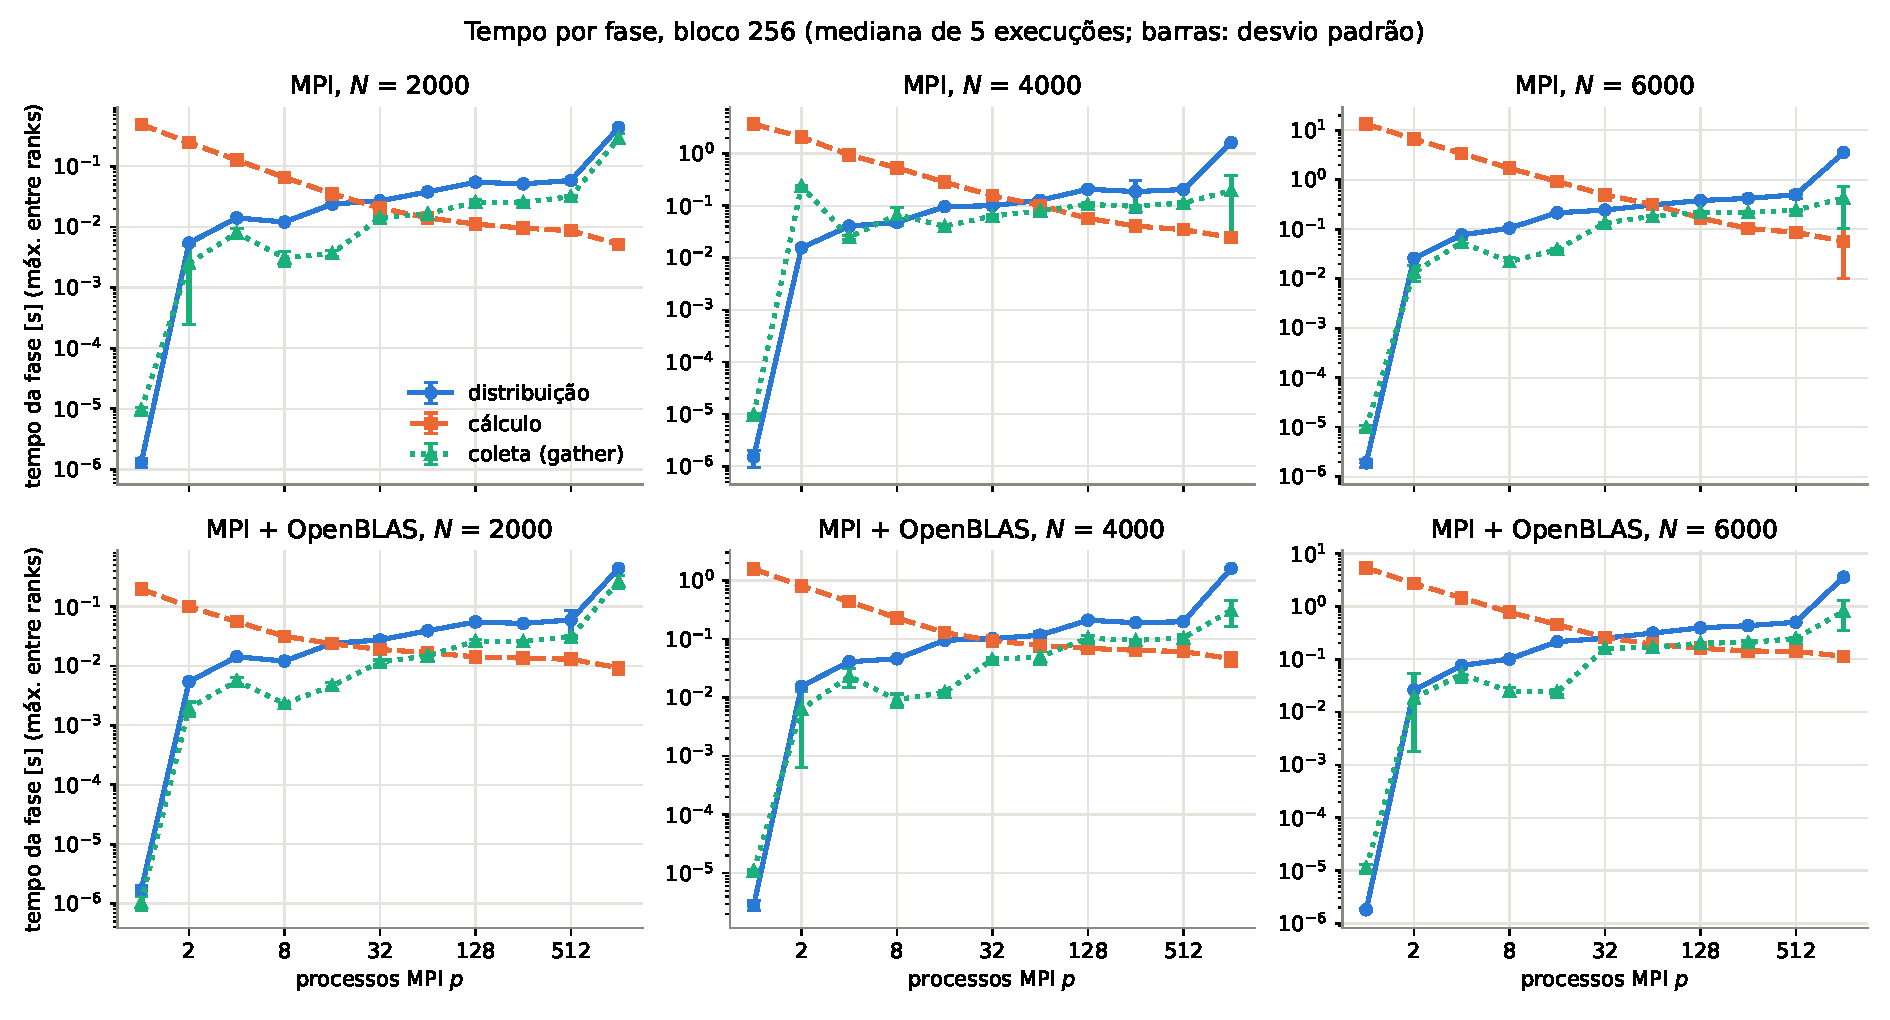
\includegraphics[width=\textwidth]{fases_b256.pdf}
\vspace{-1ex}
\caption{Tempo de cada fase da Equação~\eqref{eq:fases}, isto é, distribuição, cálculo e coleta, cada uma como máximo entre os ranks, em função de $p$, bloco 256, $N=2000$, 4000 e 6000, para a MPI em cima e a MPI + OpenBLAS embaixo, com eixos em escala logarítmica. Pontos: mediana de 5 execuções; barras: desvio padrão.}
% fonte: results/metrics.csv, metric in {time_distribution_s, time_compute_s, time_gather_s}, scaling=strong, block_size=256; gerada por scripts/make_figures.py
\label{fig:fases}
\end{figure}

\begin{figure}[!htb]
\centering
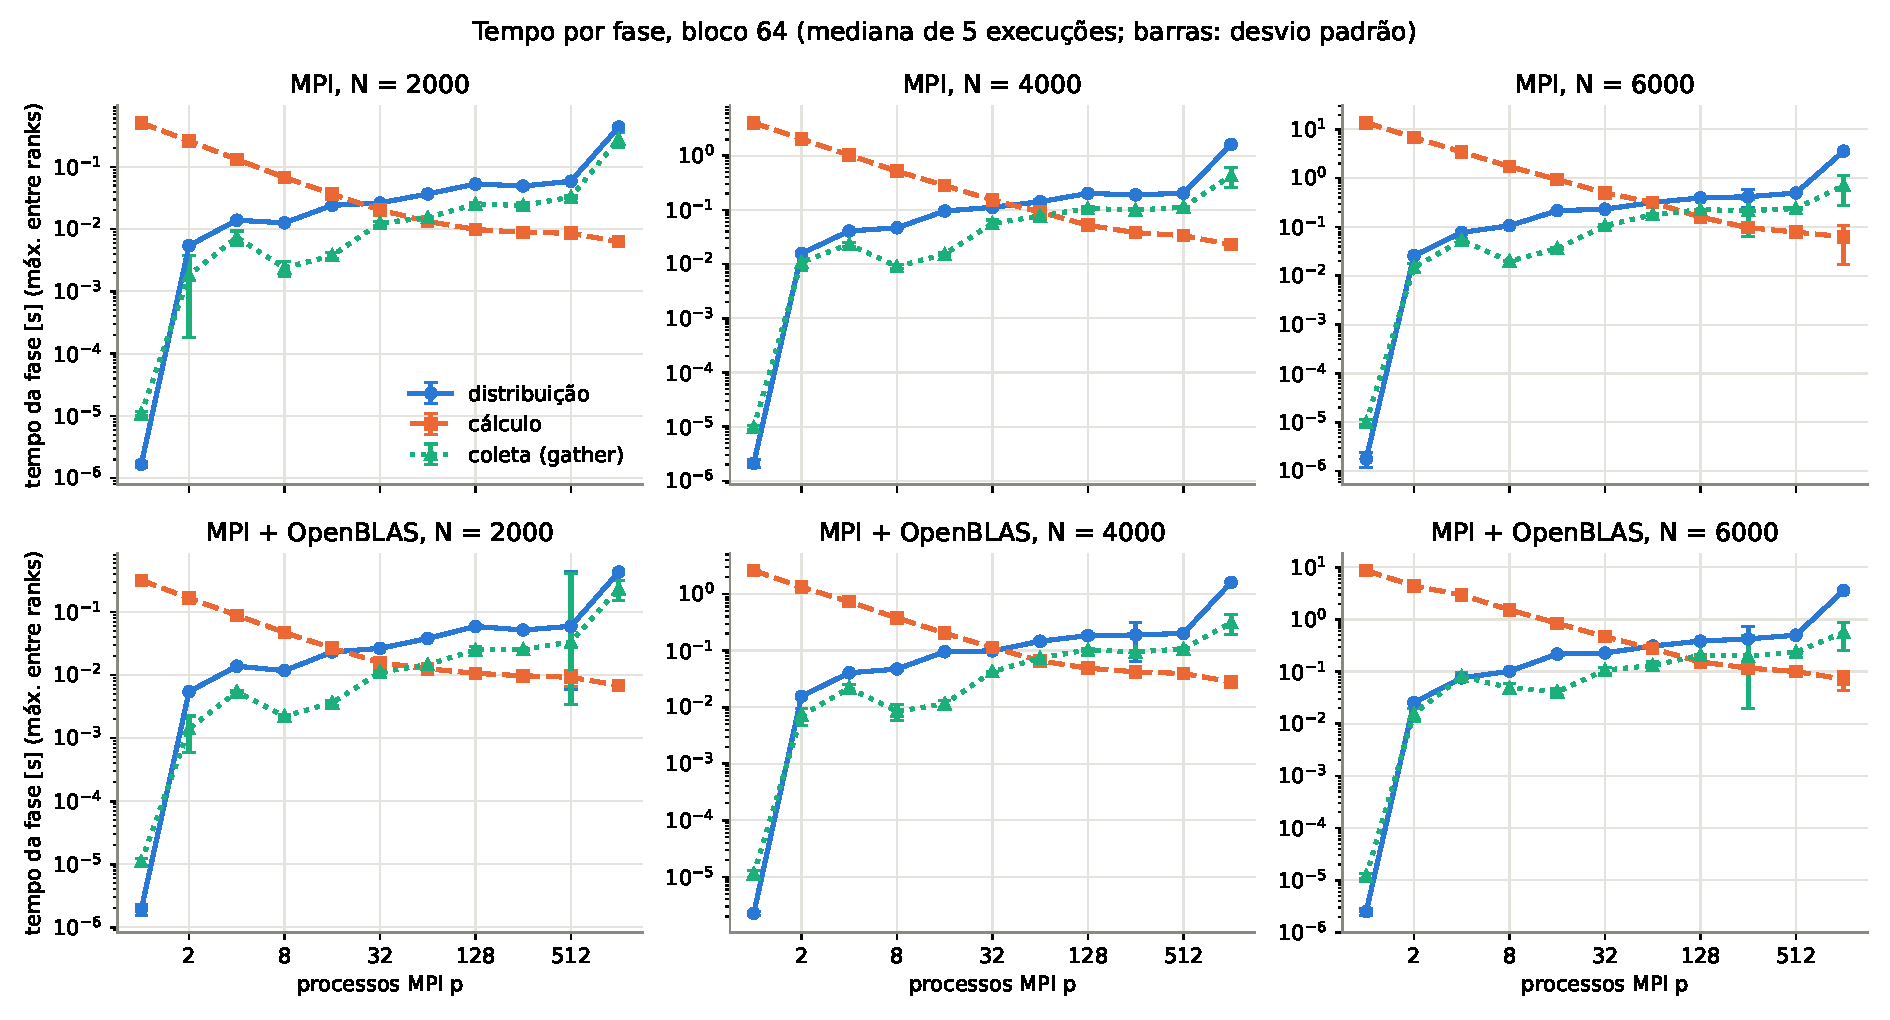
\includegraphics[width=\textwidth]{fases_b64.pdf}
\caption{Tempo de cada fase como na Figura~\ref{fig:fases}, para o bloco 64. Pontos: mediana de 5 execuções; barras: desvio padrão.}
% fonte: results/metrics.csv, metric in {time_distribution_s, time_compute_s, time_gather_s}, scaling=strong, block_size=64; gerada por scripts/make_figures.py
\label{fig:fases2}
\end{figure}

\begin{figure}[!htb]
\centering
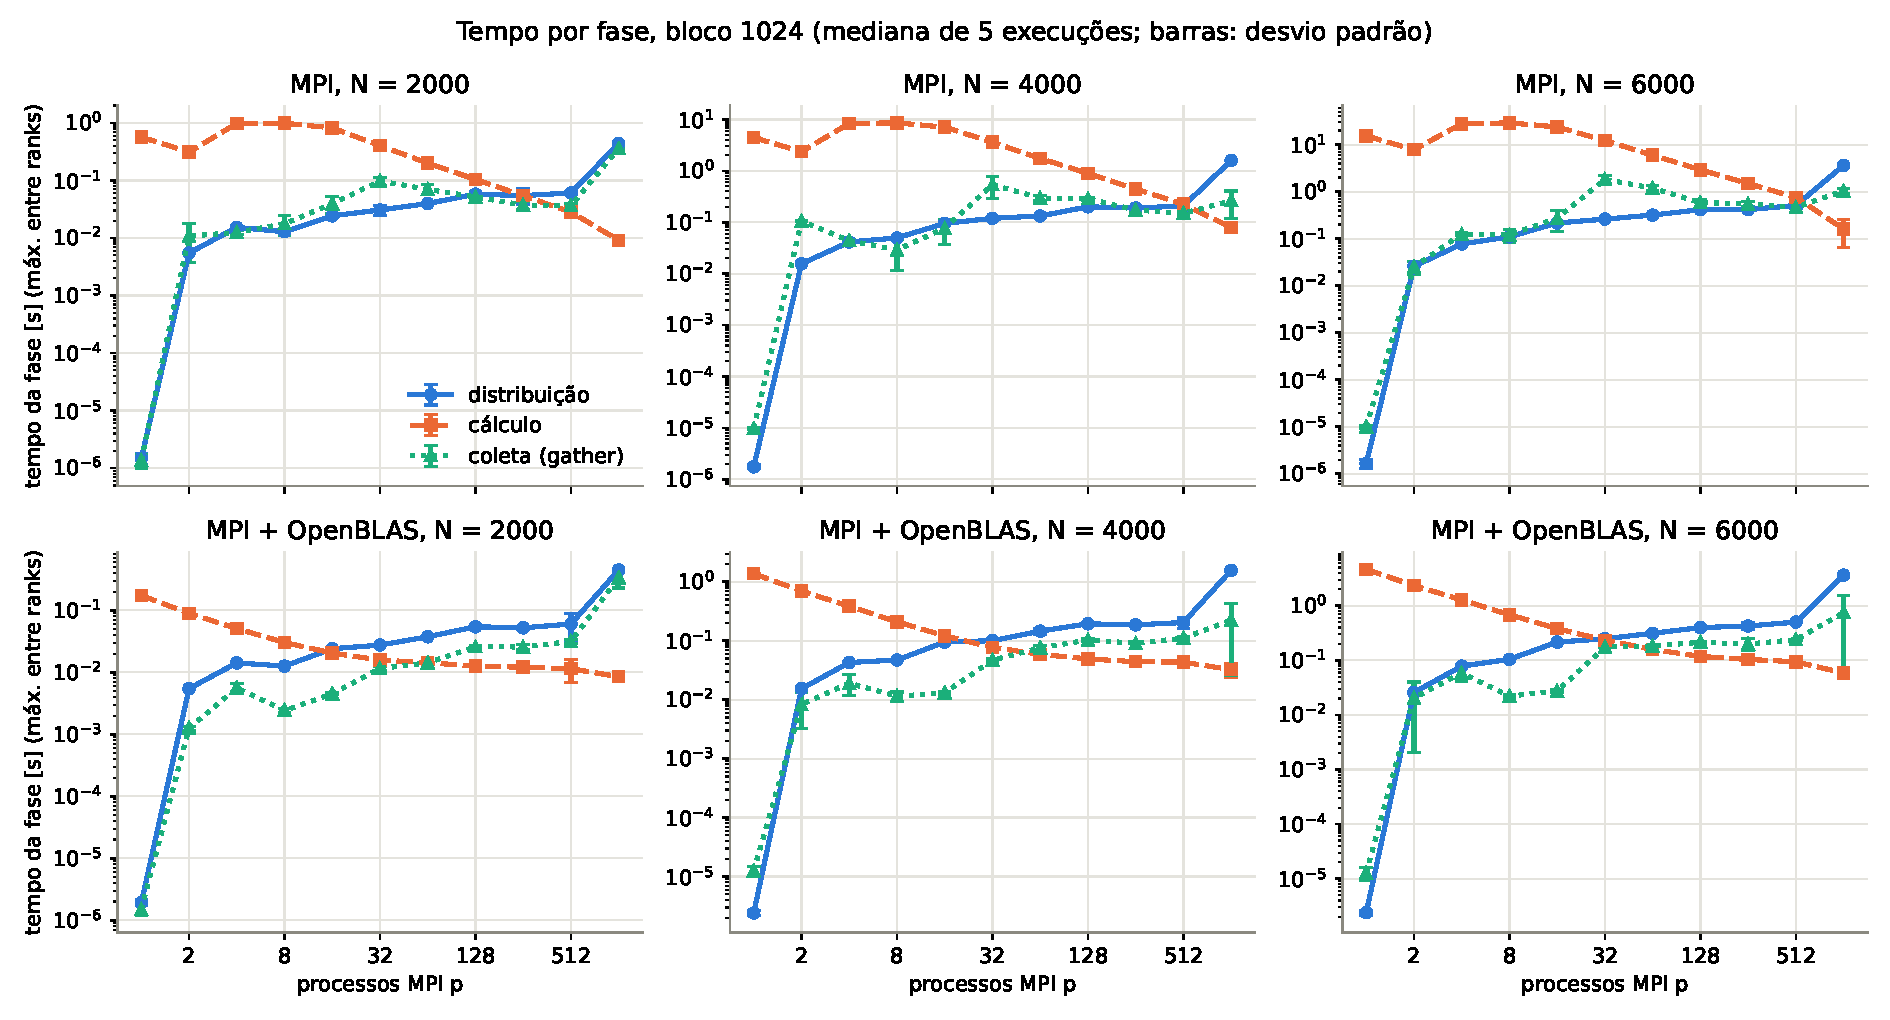
\includegraphics[width=\textwidth]{fases_b1024.pdf}
\caption{Tempo de cada fase como na Figura~\ref{fig:fases}, para o bloco 1024. Na MPI o cálculo domina até $p\approx 128$, efeito da degradação do kernel com esse bloco. Pontos: mediana de 5 execuções; barras: desvio padrão.}
% fonte: results/metrics.csv, metric in {time_distribution_s, time_compute_s, time_gather_s}, scaling=strong, block_size=1024; gerada por scripts/make_figures.py
\label{fig:fases3}
\end{figure}

\section{Discussão}
\textbf{Ganhos.} Há dois ganhos independentes. O kernel OpenBLAS sozinho, com $p=1$, dá $S^{\mathrm{tot}}_1$ de 1,56 a 1,61 com bloco 64, 2,32 a 2,46 com bloco 256 e 3,22 a 3,31 com bloco 1024. O paralelismo dá até $S_p = 26{,}5$ na MPI, com $N=6000$, $b=64$ e $p=256$, ou 25,2 com $b=256$. Combinados, o melhor speedup total medido é 32,3, da MPI + OpenBLAS com $N=6000$, $b=1024$ e $p=64$, em 0,473 s, contra 26,5 da MPI, como mostra a Tabela~\ref{tab:melhor}. A MPI + OpenBLAS tem o menor tempo absoluto nos três tamanhos, mas a menor eficiência paralela: quanto mais rápido o kernel, maior a fração do tempo gasta na comunicação, que é a mesma nas duas versões.

\textbf{Gargalo principal: a cópia completa de $B$.} Todo rank recebe $B$ inteira por \texttt{MPI\_Bcast}. Como $B$ tem $N^2$ valores \texttt{float} de 4 B, a memória ocupada pela cópia de $B$ em cada rank é
\begin{equation}\label{eq:memB}
M_B = N^2 \cdot 4\ \mathrm{B},
\end{equation}
o que dá $2000^2\cdot4 = 16$ MB, $4000^2\cdot4 = 64$ MB e $6000^2\cdot4 = 144$ MB por rank, com MB $=10^6$ B. Com 128 ranks por nó isso é $128\cdot144 = 18\,432$ MB, cerca de 18,4 GB de cópias de $B$ por nó com $N=6000$, dos 512 GB do nó. O volume total entregue pelo \texttt{Bcast} aos ranks que não são a raiz é
\begin{equation}\label{eq:bcast}
V_{\mathrm{Bcast}} = (p-1) \cdot N^2 \cdot 4\ \mathrm{B},
\end{equation}
em que $p-1$ é o número de ranks que recebem a cópia. Com $N=6000$ ele vale $127\cdot144 = 18\,288$ MB, cerca de 18,3 GB, em $p=128$ e $1023\cdot144 = 147\,312$ MB, cerca de 147 GB, em $p=1024$. Pela Equação~\eqref{eq:bcast}, esse volume cresce linearmente com $p$, enquanto o cálculo por rank cai com $1/p$; por isso a distribuição domina para $p$ grande, como mostra a Tabela~\ref{tab:fases}. Já o \texttt{Scatterv} de $A$ e o \texttt{Gatherv} de $C$ movem $N^2$ valores no total, independentemente de $p$.
% números calculados aqui: N^2 * 4 B por rank; x128 ranks por nó; (p-1) * N^2 * 4 B entregues pelo Bcast (MB = 10^6 B)

\textbf{Outros gargalos.} O primeiro é a coleta: o \texttt{Gatherv} no rank 0 inclui a espera pelo rank mais lento e chega a 0,22 s com $N=6000$ e $p=128$. O segundo é a banda de memória e o L3 compartilhados: ocupar os 128 núcleos de um nó rende pouco sobre 64 núcleos, e espalhar os mesmos 128 processos em 2 nós é até 1,49 vezes mais rápido, ou 1,52 vezes em 8 nós. O terceiro é a comunicação entre nós em grande escala: em $p=1024$, com 8 nós, a distribuição leva 3,56 a 3,64 s com $N=6000$, e $f_{\mathrm{com}}$ fica entre 0,95 e 0,99 em todos os tamanhos. O quarto é o bloco 1024 no kernel em C, que degrada a MPI de $p=4$ a 32. Uma distribuição 2D, como SUMMA ou Cannon, em que cada rank guarda só $N^2/\sqrt{p}$ elementos de $B$, reduziria o gargalo principal; ela não foi implementada.

\section{Limitações}
\begin{itemize}\setlength{\itemsep}{0pt}
\item Núcleos e processos nunca foram separados: sempre 1 rank por núcleo com 1 thread de OpenBLAS; não há execuções híbridas MPI $\times$ threads nem OpenBLAS multithread sem MPI. A versão Serial só existe com $p=1$, e não há linha de base OpenBLAS sem MPI; a MPI + OpenBLAS com $p=1$ é o substituto mais próximo.
\item Acima de 128 processos, $p$ e o número de nós mudam juntos, com 128 processos por nó e um único ponto por número de nós. O efeito dos nós com $p$ fixo só foi medido com $p=128$, e o ponto de 1 nó vem de outro job, fila e host que os de 2, 4 e 8 nós: o job 1034860, na fila \texttt{par128}, em \texttt{adano35}, contra o job 1034865. A variação entre hosts não foi quantificada, o que pode explicar o desvio do ponto de 4 nós.
\item A escalabilidade fraca tem só 3 pontos, $p=1$, 8 e 27, em 1 nó; a sua referência com $p=1$ é uma execução própria, por exemplo 0,50799 s para MPI com bloco 64, e não a da série forte, de 0,509047 s.
\item Só os blocos 64, 256 e 1024 foram medidos; o caso sem ladrilhos, com $b=0$ e uma única \texttt{sgemm} com o bloqueio interno do OpenBLAS, só aparece nos testes de corretude.
\item A variabilidade vem de 5 execuções por configuração, num único job por configuração, sem intervalos de confiança; o desvio padrão é inflado por execuções lentas isoladas, todas na distribuição dos jobs multinó.
\item Os tempos por fase são máximos independentes entre os ranks; \texttt{Scatterv} e \texttt{Bcast} não são medidos separadamente, e o desbalanceamento entre ranks não foi registrado. O rótulo de $f_{\mathrm{com}}$ no \texttt{metrics.csv} está desatualizado, como explica a Seção~\ref{sec:proc}.
\item O GFLOP/s usa o tempo total; não há pico teórico, contadores de hardware, \emph{roofline} nem perfil, por isso as explicações da degradação com bloco 1024 e do ponto de 4 nós são hipóteses. A interconexão física entre os nós e o transporte usado pelo Open MPI não foram registrados nos logs; sabe-se apenas que a PML \texttt{ucx} está disponível.
\item Rastreabilidade do código: o log de compilação registra a revisão \texttt{48314089}, e os logs de ambiente dos jobs de medição registram \texttt{0cd7312b}, no job 1034860, e \texttt{d3d48870}, nos jobs 1034858 e 1034865. Nenhuma dessas revisões está no histórico local atual do repositório, que foi reescrito. A correspondência exata entre código e medições é, portanto, parcial; o código medido corresponde ao estado publicado no commit \texttt{ace5e73}.
% fonte: results/logs/build_1034701.log:12; results/logs/1034860_single_node/environment.log:113-114;
% results/logs/1034858_multi_node/environment.log:120-121; results/logs/1034865_node_sweep/environment.log:120-121; git cat-file no repositório
\end{itemize}

\section{Compilação e execução}
O código, os scripts e as instruções completas estão no README do repositório \href{https://github.com/oliveiraMats2/HPC_Matrix_Multiplication}{github.com/\allowbreak oliveiraMats2/\allowbreak HPC\_Matrix\_\allowbreak Multiplication}. A compilação usa CMake com o preset \texttt{lovelace}, que define \texttt{CMAKE\_C\_COMPILER=gcc}, \texttt{MATMUL\_ARCH\_FLAGS=-march=znver2} e \texttt{Release} e liga MPI, OpenBLAS e testes; no cluster, ela é feita num nó de cálculo pelo \texttt{build.pbs}. Todos os jobs carregam o mesmo ambiente com \texttt{scripts/env\_lovelace.sh}. Os comandos, executados na raiz do repositório, são:

{\footnotesize
\begin{alltt}
# ambiente: scripts/env_lovelace.sh, carregado por todo job PBS
module purge
module load gcc/9.4.0 openmpi/4.1.1-gcc-9.4.0 openblas/0.3.21-gcc-9.4.0
module load cmake/3.26.3-gcc-9.4.0              # só na compilação
export CC=gcc OPENBLAS_NUM_THREADS=1 OMP_NUM_THREADS=1

# compilação e testes, o mesmo que qsub scripts/build.pbs faz num nó de cálculo
cmake \dd{}preset lovelace                        # -O3 -march=znver2
cmake \dd{}build \dd{}preset lovelace -j
ctest \dd{}preset lovelace

# submissão no Lovelace
qsub scripts/build.pbs          # fila testes: compilação + ctest
qsub scripts/smoke.pbs          # fila testes: N = 256/300, p = 1-4, captura de erro
qsub scripts/run_par128.pbs     # 1 nó exclusivo: serial, forte p = 1..128, fraca 1/8/27
qsub scripts/run_paralela.pbs   # 8 nós exclusivos: forte p = 256/512/1024 em 2/4/8 nós
qsub scripts/run_nodes.pbs      # 8 nós exclusivos: p = 128 fixo em 2/4/8 nós
python3 scripts/analyze_results.py               # métricas, tabelas e figuras

# linha de lançamento usada em cada execução, de scripts/run_benchmarks.sh
mpirun -np P \dd{}map-by core \dd{}bind-to core \textbackslash
    env OPENBLAS_NUM_THREADS=1 OMP_NUM_THREADS=1 \textbackslash
    build/lovelace/matmul_mpi_openblas \dd{}config config.toml \dd{}size N \dd{}block B \textbackslash
    \dd{}repetitions 1 \dd{}warmup 1 \dd{}run-offset R \dd{}scaling strong \dd{}csv results/benchmark.csv
\end{alltt}}

Os cabeçalhos PBS pedem nós inteiros e exclusivos: \texttt{run\_par128.pbs} usa \texttt{-q par128} e \texttt{select=1:ncpus=128:mpiprocs=128}; \texttt{run\_paralela.pbs} e \texttt{run\_nodes.pbs} usam \texttt{-q paralela} e \texttt{select=8:ncpus=128:mpiprocs=128}; os três usam \texttt{place=scatter:exclhost}. Os parâmetros do experimento ficam em \texttt{config.toml}; os principais são:

{\footnotesize
\begin{alltt}
[experiment]   matrix_sizes = [2000, 4000, 6000]   repetitions = 5   warmup = 1   seed = 42
[blocking]     block_sizes = [64, 256, 1024]
[mpi]          process_counts = [1, 2, 4, 8, 16, 32, 64, 128]
               multinode_process_counts = [256, 512, 1024]   distribution = "row_block"
[weak_scaling] matrix_sizes = [2000, 4000, 6000]   process_counts = [1, 8, 27]
[openblas]     threads = 1
[benchmark]    absolute_tolerance = 0.001   relative_tolerance = 0.0001
[cluster]      expected_cpu_model = "AMD EPYC 7662"   cores_per_node = 128
\end{alltt}}

O número de nós não está no TOML: vem da linha \texttt{select=} do PBS e do \emph{hostfile} de cada lançamento, e é gravado em cada linha do CSV.

\end{document}
